\documentclass[twoside, master]{NJUthesis}
% \documentclass[pdftex]{NJUthesis}

% 可选参数:
%   nobackinfo 取消封二页导师签名信息
%   oneside/twoside 单面/双面打印
%   phd/master 博士/硕士论文
% 下面三个选一个:
% dvipdfm 使用 dvipdfm(x) 生成最终的 PDF 文档 (缺省设置,不建议修改)
% dvips 使用 dvips 生成最终的 PS 文档
% pdftex 使用 pdfLaTeX 生成最终的 PDF 文档

%%%%%%%%%%%%%%%%%%%%%%%%%%%%%%
%% 导言区
%%%%%%%%%%%%%%%%%%%%%%%%%%%%%%

% 小节标题靠左对齐
\CTEXsetup[format+={\flushleft}]{section}

% 设置链接颜色
\hypersetup{
% pdf 属性
             pdftitle={LaTeX Thesis Template of Nanjing University}, %
            pdfauthor={Jia Nie}
}

% 表格
\usepackage{longtable, multirow}
% 英文使用 Times 字体
\usepackage{times}
% 源代码
\usepackage{fancyvrb}
% 自定义列表样式
\usepackage{enumitem}

\usepackage{amsmath}
\usepackage{amssymb}
\usepackage{moreverb}
\usepackage{txfonts}
\usepackage{mathcomp}
\usepackage{graphicx}
\usepackage{subfigure}
\usepackage[linesnumbered,boxed,ruled,vlined]{algorithm2e}
\usepackage{array}
\usepackage{multirow}

%%	added by Jiang
\usepackage{extarrows}	%使用长箭头
\usepackage{nomencl}	%与术语表有关的包

\usepackage{booktabs}
\usepackage{float}

\makenomenclature

\setcounter{topnumber}{5}

\theoremstyle{plain}
\newtheorem{definition}{\hspace{2em}定义}[chapter]
\newtheorem{lemma}{\hspace{2em}引理}[chapter]
\newtheorem{theorem}{\hspace{2em}定理}[chapter]
\newtheorem{property}{\hspace{2em}性质}[chapter]
\newtheorem{example}{\hspace{2em}例}[chapter]
\newtheorem{myrule}{\hspace{2em}规则}[chapter]


\newcommand{\tabincell}[2]{\begin{tabular}{@{}#1@{}}#2\end{tabular}}% 表格内换行
\renewcommand{\footnoterule}{%脚注线
  \kern -3pt
  \hrule width 2.3in height 0.4pt
  \kern 2pt
}


\begin{document}

%%%%%%%%%%%%%%%%%%%%%%%%%%%%%%
%% 封面部分
%%%%%%%%%%%%%%%%%%%%%%%%%%%%%%

% 国家图书馆封面内容字符串
% 仅博士需要填写并保证模板参数选择了 phd
\classification{}
\confidential{}
\UDC{}
\titlelinea{南京大学学位论文}
\titlelineb{~\LaTeX{}~模板}
\titlelinec{}
\advisorinfo{南京大学~计算机系}
\chairman{XXX 教授}
\reviewera{某某某某 副研究员}
\reviewerb{XXX 教授}
\reviewerc{XXX 教授}
\reviewerd{XXX 教授}
\nlcfootdate{~年~~月~~日}

% 南大中文封面内容字符串
\title{test}
% \title{基于代码依赖关系的需求与代码的一致性维护方法研究}
% \author{\kaishu聂佳}
% \studentnum{MF1333034}
% \grade{2013}
% \advisor{\kaishu胡昊~~副教授}
% \major{\kaishu计算机技术}
% \researchfield{\kaishu软件方法学}
% \footdate{\kaishu2016~年~5~月}
% \submitdate{\kaishu2016~年~5~月~26~日}
% \defenddate{\kaishu2016~年~5~月~26~日}

% 英文封面内容字符串
\englishtitle{Research on Composite Service Skyline with QoS Correlations}
\englishauthor{Yu Du}
\englishadvisor{Associate Professor }
\englishadvisorname{Hao Hu}
\englishinstitute{Institute of Computer Software }
\englishdegree{Master of Engineering}
\englishmajor{Computer Software and Theory}
\englishdate{May 2016}
% 制作封面命令
% \maketitle

% \makechinesetitle

% 制作英文封面命令
\makeenglishtitle


%%%%%%%%%%%%%%%%%%%%%%%%%%%%%%
%% 前言部分
%%%%%%%%%%%%%%%%%%%%%%%%%%%%%%
\frontmatter

% 中文摘要
% \begin{abstract}

% \keywords{服务组合,QoS~关联,组合服务~Skyline,移动Web服务,剪枝,安全值范围}

% \end{abstract}

\begin{englishabstract}

在软件维护与演化的过程中,一份与代码实现相一致的需求规约能够提供有价值的信息以支持维护与演化任务的完成。然而,对需求规约的更新仍然是一项手工任务,需要付出较高的人工与时间成本。因此,维护人员通常直接更新代码,而不更新需求。这将导致需求的过时与失效,从而使软件系统的可维护性减弱。

在代码更新后,识别代码变更所影响的潜在过时需求,能够帮助维护人员保持需求规约与代码实现的一致性。在软件工程领域,需求可追踪性是直接关联需求与代码的主要方式。但在实际中,需求可追踪性的使用有限,这是由于建立与维护需求与代码间完备的追踪关系代价高昂。因此,现有工作从分析代码变更的角度出发,识别其中影响需求的变更代码并构造其文本描述,并基于信息检索技术匹配变更代码描述与需求的文本,以发现需求规约中受影响的部分需求。然而,基于信息检索的方法存在词汇失配问题,导致方法的精度有限。如何提高受影响需求检测方法的精度是当前研究的重点。现有工作主要关注代码的变更部分,而变更部分通常只包含局部信息,与变更部分在结构上有依赖关系的上下文信息同样有价值。同时,在需求可追踪性,特征定位和概念分配等相关领域,代码依赖关系已经被用于与代码的文本信息相结合,以提高领域内方法的效果。然而,上述工作在分析代码依赖关系时,假设所有的代码依赖关系是同样重要的,没有对各个依赖关系的重要性加以区分,从而无法充分发挥代码依赖关系的作用。此外,对于被检测需求,维护人员可能仍然需要需要与变更有关的知识以完成对需求的更新。

针对上述问题,本文完成了以下工作:
\begin{enumerate}
  \item 我们提出了一种代码依赖关系的紧密度分析方法,以区分代码依赖关系的重要性。同时,我们将此分析方法应用于需求可追踪性生成问题,提出了一种改进的需求到代码间追踪关系的生成方法TRICE(Traceability Recovery based on Information retrieval and ClosEness analysis),并在三个实验系统下验证了TRICE的有效性。
  \item 在依赖关系紧密度分析有效性被验证的基础上,我们提出了一种基于代码依赖关系的过时需求自动检测与更新推荐方法,通过对代码依赖关系的紧密度分析,引入了与变更代码在结构上有紧密依赖的上下文代码信息。同时,方法能够推荐与需求更新相关的变更代码元素。我们在三个研究案例下设计并完成实验,验证了方法的有效性。
  \item 我们实现了一个过时需求自动检测工具INFORM(IdeNtiFy Outdated RequireMents),并集成了基于代码依赖关系的过时需求自动检测与更新推荐方法,以辅助维护人员进行需求更新。
\end{enumerate}

\keywords{服务组合,QoS~关联,组合服务~Skyline,移动Web服务,剪枝,安全值范围}

\end{englishabstract}

% 英文摘要
\begin{englishabstract}

When maintaining and evolving software, a requirements specification which is consistent with the code implementations provides valuable knowledge for supporting several maintenance and evolution tasks. However, updating the requirements is still a manual task that is expensive and time consuming. Therefore, maintainers usually change the code directly and leave the requirements unchanged. This leads to requirements rapidly becoming outdated and useless, then weakening the maintainability of software system. 

By identifying the impacted requirements when code is changed, the potential outdated requirements can facilitate the effort to keep the consistency between requirements specification and code implementations. In software maintenance, the main approach for contacting requirements with code is traceability. In practice, the use of traceability is limited because of the cost to completely tracing requirements to code is expensive. Therefor, from the perspective of code changes, the existing work first recognize the code changes which are impacting the requirements and construct textual descriptions for these changes, then using IR-based approach to tracing change descriptions to requirements in order to find the impacted parts of requirement specifications. However, the accuracy of IR-based approach is limited because of the vocabulary mismatch problem. Improving the accuracy of detecting impacted requirements is the main point for current research. Existing work focus on the changed parts of code but the changed parts usually contain only local information, the contexts which have structural dependencies with the changed ones may also provide valuable information. Meanwhile, in related fields like traceability, feature location and concept location, code dependencies have been proved to be valid for improving the corresponding approaches by combining with textual information. However, mentioned works assume that all code dependencies are equally important and limit the advantages of code dependencies. Besides, facing with the detected requirements, maintainers may still need more knowledge which is related with the code changes to finish updating the requirements.

For the above problems, we finished several works as following:
\begin{enumerate}
  \item We proposed an approach to measure the closeness of code dependencies. Moreover, we applied it to generate trace links between requirements and code, we proposed an enhanced approach called TRICE (Traceability Recovery based on Information retrieval and ClosEness analysis), and we evaluated TRICE on three different software systems.
  \item As the evaluated effectiveness of closeness analyzing, we proposed an approach based on code dependencies to automatically detect outdated requirements and recommend knowledge about changes. We bring the contexts which are tight with the changed code in structure by analyzing the closeness of code dependencies. Meanwhile, our approach can recommend relevant code elements for updating requirements. We evaluated the approach on three different case studies.
  \item We also develop a tool called INFORM (IdeNtiFy Outdated RequireMents) and integrating the above approach to help maintainers updating requirements.
\end{enumerate}
\englishkeywords{Service composition, QoS correlation, Composite service skyline, Mobile Web service, Pruning, Safe value range}

\end{englishabstract}

% 生成目录命令
\tableofcontents

% 以下两个目录可根据具体情况注释掉
% 生成表格目录命令
%\listoftables
% 生成插图目录命令
\listoffigures

%生成术语表命令
%\include{chapter/Nomenclatures}
%\def\nomname{缩略语对照表}
%\printnomenclature[5em]



%%%%%%%%%%%%%%%%%%%%%%%%%%%%%%
%% 正文部分
%%%%%%%%%%%%%%%%%%%%%%%%%%%%%%
\mainmatter

\chapter{绪言}

\section{研究背景}

\section{研究现状}

\section{本文工作}

\section{本文组织}


\chapter{相关工作}

\section{需求可追踪性的相关概念}

\subsection{基本概念}

在软件工程领域,人们认为应该要追踪一个需求使用期限的全过程,编制每个需求同系统元素之间的联系文档,这样的关联关系提供了需求到产品整个过程范围的明确的查阅能力,需求可追踪性(Traceability)概念的提出,正是为了应对上述问题。1970年,需求可追踪性被列入美国国防部合同条款;1992年,经过软件工程领域内的广泛讨论被认为有助于软件开发实践;1994年,需求可追踪性有了如下的明确定义\cite{gotel1994analysis}:

定义:需求可追踪性是指,在软件生命周期中,对某一特定需求形成以及演变的追踪能力,既包括后向追踪,从需求文档确定后一直到软件发布过程中的各种制品之间的追踪(例如设计文档、代码和测试)又包括前向追踪,书写文档形式的需求追踪到需求的来源。

无论是正向追踪或是反响追踪,我们都可以用一个二维矩阵将对应关系固化。以需求与代码间的追踪关系为例,图N为对应的需求追踪矩阵。其中,列表示需求项,行表示代码项,矩阵间的标记表明对应列的需求与对应行的代码存在关联关系,既此代码负责实现该需求描述的行为,在实际的软件生产过程中,需求的粒度可以是用例(Use Case)或声明(Requirement Statement),对于面向对象的程序,代码的粒度通常是类或者函数。

\begin{table}[]
\centering
\caption{需求追踪矩阵(需求到代码)}
\label{my-label}
\begin{tabular}{@{}cccccc@{}}
\toprule
      & $Requirement_{1}$ & $Requirement_{2}$ & $Requirement_{3}$ & ... & $Requirement_{n}$ \\ \midrule
$Code_{1}$ & X            &              &              &     &              \\
$Code_{2}$ &              & X            &              &     &              \\
$Code_{3}$ & X            &              &              &     & X            \\
$Code_{4}$ &              &              & X            &     & X            \\
...   &              &              &              &     &              \\
$Code_{n}$ &              & X            &              &     &              \\ \bottomrule
\end{tabular}
\end{table}

\subsection{研究现状}

Maeder等人\cite{mader2012assessing}分析了需求可追踪性对于软件维护任务的有益程度,他们通过研究案例iTrust与Gantt的实验,分析认为在需求可追踪性的辅助下,维护任务平均能够提高21\%的效率与60\%的准确度。然而,追踪关系的建立和维护需要也需要成本,只有当收益高于成本时,追踪关系的实施才有现实意义。文章\cite{mader2012assessing}同时分析了收益成本间的关系,分析显示随着软件演化,当维护任务达到一定数量时,在需求可追踪性的辅助下能够减少维护任务的总成本。

尽管如此,真实世界的软件系统中通常缺少固化的追踪关系\cite{ramesh1995implementing},这主要是由于(1)追踪关系在软件开发的过程中难以捕获。要求开发者在实现软件功能的同时建立和维护追踪关系代价较高,开发者实施追踪关系的意愿不高;(2)追踪关系在软件开发完成后难以重建。对于一个完成的软件系统,早期参与的开发者可能已经不在项目组中,或是遗忘系统的实现细节,导致重建追踪关系的困难。因此,领域内希望通过增强过程的自动化程度以辅助开发者完成追踪关系的生成。

目前领域内主流生成追踪关系的方法是从Antoniol等人\cite{antoniol2002recovering}的奠基性工作发展而来,该工作利用基于VSM(向量空间模型)的方法检索需求和代码间的追踪关系。方法核心在于利用信息检索技术估计文本间的相似度。继承这一想法的工作\cite{marcus2003recovering,cleland2005utilizing}分别选用LSI(潜在语义索引),JS(概率模型)检索需求和代码间的追踪关系,而比较三者模型发现,没有一种检索模型占有明显优势\cite{abadi2008traceability,eaddy2008cerberus}。

尽管基于信息检索的方法能够完全自动化的生成追踪关系,但是此类方法的精度(准确率,召回率)有限。这是由于基于文本匹配的信息检索存在词汇失配(Vocabulary Mismatch)的问题。代码的文本质量低,同义词问题等情况都会影响检索的精度。因此,出现了一系列的工作对基于信息检索的追踪关系生成方法进行改进。Dasgupta等人\cite{dasgupta2013enhancing}通过引入与代码相关的文档扩展以扩展文本的内容;Ali等人\cite{ali2012empirical}利用Eye-Tracking设备追踪维护人员在建立追踪时的眼球轨迹,以发现对维护人员重要的代码实体,并根据代码实体的重要性(函数>注释>变量>类)为来自代码实体的词项赋权;在 Ali等人\cite{ali2013trustrace}的另一份工作中,通过挖掘软件生产过程以提供额外的信息源(Commit,Bug Report,Mail List)参与决策
;Mahmoud\cite{mahmoud2013supporting}等人通过重构代码的方式改善了代码文本的质量,以减轻词汇失配的程度。Capobianco\cite{capobianco2013improving}等人则认为在检索时名词能够提供最为关键的信息,而形容词和副词等会带来干扰;Diaz等人\cite{diaz2013using}提出利用代码所有权的概念提高追踪关系的检索精度。

上述方法主要是通过引入额外文本信息或对文本赋权的方式以弥补原有需求、代码文本质量的不足。而代码与需求不同,除了文本信息之外,代码还包含结构信息,另一类工作通过深入挖掘代码的结构信息以提高追踪关系的检索精度。McMillan等人\cite{mcmillan2009combining}结合代码的文本和结构信息用于追踪关系的生成,在基于文本信息检索的候选追踪关系之上,利于结构信息进行追踪关系的重排序;Panichella等人\cite{panichella2013and}认为如果候选追踪关系本身的精度较低,则基于代码结构信息的重排序可能起到反效果,因此提出在用户反馈阶段使用代码结构信息。

\section{基于信息检索的需求到代码间追踪关系生成技术}

在需求与软件过程的各种制品之间的关联关系中,需求与代码的关联关系引起了开发者的主要关注,这是由于需求描述了与软件系统行为有关的高层概念,而代码负责软件系统行为的实现,两者的关联关系能够帮助开发者理解程序,分析需求变更的影响性,完成包括维护任务、二次开发,代码复用在内的一系列软件活动。

\begin{figure}[thb]
    \centering
    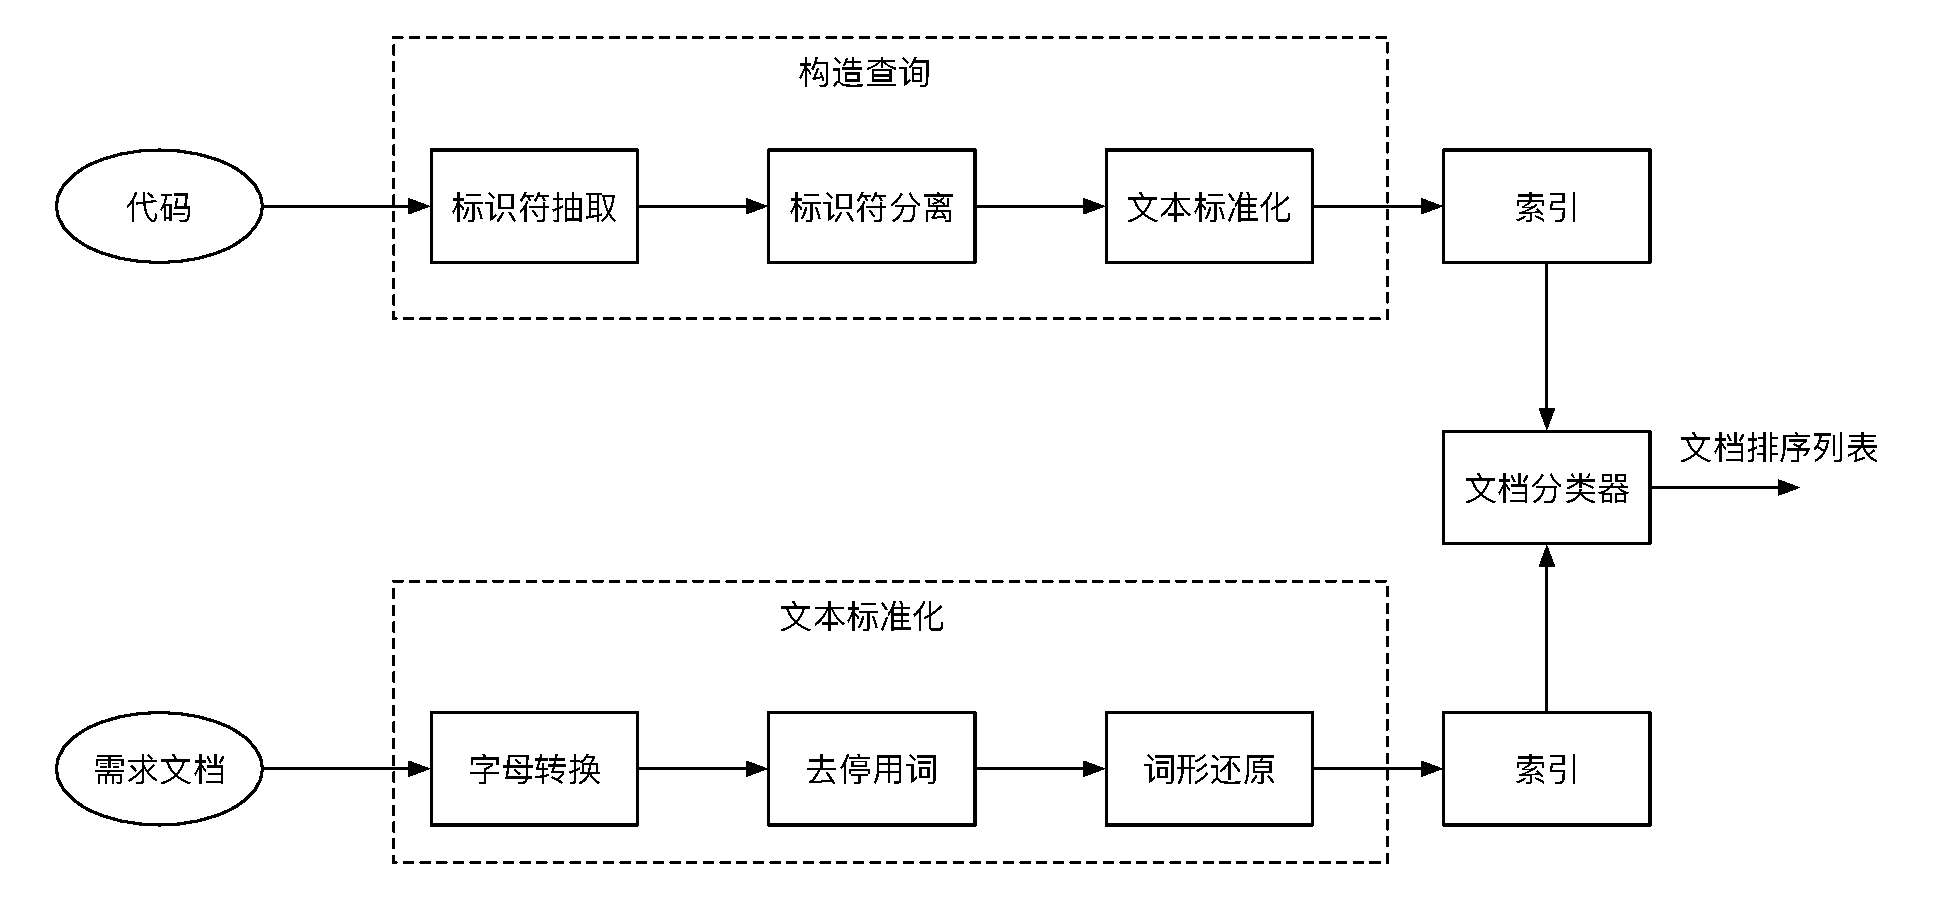
\includegraphics[width=1.0\textwidth]{./figures/related_work/ir_traceability_process.pdf}
    \caption{追踪关系生成方法}
    \label{F:BuildLogScrn}
\end{figure}

\subsection{追踪关系生成方法}

Antoniol等人\cite{antoniol2002recovering}提出了基于信息检索的需求到代码间追踪关系生成方法。方法的核心想法是,假设代码中标识符的命名有意义,或与需求文档共用同一个术语表,因此能够通过文本匹配的方式建立需求和代码的关联关系。方法的基本过程如图N所示。在进行需求和代码的检索前,方法首先通过两条路径(需求文档到文档,代码到查询)构造文档与查询。

在构造文档这一路径,基于文档中抽取的词能够建立文档的索引,词的构造与索引的建立需要通过以下三个步骤的文本标准化处理:
\begin{enumerate}
  \item 将文档中的字母统一转换为小写。

  \item 根据停用词表删去文档中的停用词,通常停用词包括(标点、数字、介词等)。

  \item 词形还原,包括将名词的复数形式转换为单数形式,将包含时态的动词还原为动词原形。
\end{enumerate}
在构造查询这一路径,方法将每个代码组件(通常是类或函数)作为一个查询,查询的构造包括以下三个步骤:
\begin{enumerate}
  \item 解析代码文本,提取代码组件的标识符。

  \item 根据标识符的命名规则(驼峰命名法,下划线分割命名法),将标识符分隔为若干独立词项。例如,标识符AmountDue,amount\_due将被分隔为词amount,due。

  \item 利用对文档进行标准化处理的三个步骤处理文本。
\end{enumerate}
最终,通过文本分类器计算查询和文档间的相似度,并返回需求到代码的候选追踪关系列表,列表根据需求文档和代码的相似度值倒序排列。显然,排序的结果与方法采取的信息检索模型有关,我们将会对三种信息检索模型(VSM,LSI与JS)进行介绍,VSM模型将查询和文档看作向量,文档根据计算的向量间距离排序;LSI在VSM的基础上,通过奇异值分解以识别词句间隐性的关联关系的模式;JS属于概率模型,估计文档与查询相关的概率,对文档根据关联概率进行排序。后续小节中将会对这三个检索模型进行详细阐述。

\subsection{信息检索模型}

\subsubsection{VSM}
VSM(Vector Space Model)是现代信息检索系统中比较常用的检索模型,它的思想是将文档与查询都看作是高维空间中的一个向量,每个维度都是一个独立的词项。

如果某个词项出现在了文档中,那它在向量中的权重就非零。常见的权重计算方法为TF-IDF,其中,TF(term frequency)是指给定的某一个词项在文本中的出现频率,IDF(inverse document frequency)用于度量词项的普遍重要性。根据直觉,对于查询中的某一个词项,如果在文档A中的出现次数多于文档B,那么文档A比B对于查询更相关。但是这里有一个缺陷在于,内容长的文档比内容短的文档有优势,长的文档总的来讲包含的词项要多些。因此我们根据文档的长度,对词项次数进行归一化,将词项次数除以文档的总词项数,这个商称为“词项的频率”,可以作为词项的局部权重。除了局部权重以外,如果一个词项只在很少的文档中出现,那么通过它就容易定位目标,应该赋予该词项较高的权重。反之,如果一个词项在大量文档中出现,则表明该词项缺少独特性,它的权重就应该较小。我们用“逆文本频率指数”(IDF)来衡量词项的全局权重。TF-IDF的计算公式如下:
\begin{align}
    tf_{i,j}=\dfrac {n_{i,j}} {\sum _{k}n_{k,j}}
  \end{align}
  \begin{align}
    idf_{i}=\log \dfrac {\left| D\right| } {\left| j:t_{i}\in d_{j}\right| }
  \end{align}
   \begin{align}
    tfidf_{i,j}=tf_{i,j} \times idf_{i}
  \end{align}
其中,$tf$指给定的某一个词项在文档中的出现频率。$n_{i,j}$为词项$t_{i}$在文档$d_{j}$中的出现次数,分母表示在文档$d_{j}$中所有词项的出现次数之和;$\left| D\right|$表示文档库中的文档总数,表示包含词项$t_{i}$的文档数目。

相似度计算是基于这样一个假设,词是文本的载体,文本的信息和词的语义是联系在一起的,也就是说同一类文本用词是相似的,不同类的文本用词各不相同。由于向量空间模型将文档与查询都看作是高维空间中的一个向量,查询与文档的相似性可基于它们在向量空间中的夹角来衡量。给定查询向量$q$, 文档向量$d$, 向量长度均为$n$, 那么其余弦相似度定义为:
\begin{align}
    sim(d_{j},q)=\dfrac {\sum _{i=1}^{n}w_{i,j} \times w_{i,q}} {\sqrt {\sum _{i=1}^{n}w_{i,j}^{2}} \ \times \sqrt {\sum _{i=1}^{n}w_{i,q}^{2}}}
  \end{align}
其中,w表示对应文档中由TF-IDF计算而来的词项权重。

\subsubsection{LSI}
LSI(Latent semantic indexing,潜在语义索引)\cite{deerwester1990indexing,dumais1991improving}在VSM的基础上通过分析词句的使用模式,以发现词句间潜在的联系。
LSI在自然语言文本中的应用表明\cite{berry1992large,landauer1997solution},LSI不仅可以捕获独立词语的含义,而且可以捕获短语(词组,句子)的含义。LSI的核心想法是,在同样的语境中出现的词语存在某些相互约束,限定了这些词之间一半具有相似的含义。在经典的文本分析应用中,LSI使用给定的语料创建词项-文档矩阵(Term-by-Document matrix),并采用奇异值分解\cite{salton1986introduction}的方式构造词项-文档矩阵的子空间,称之为LSI子空间。新的查询、文档向量通过将VSM空间的相关向量投影至LSI子空间生成。

奇异值分解背后的形式化较为复杂,详细内容可参考文献\cite{salton1986introduction}。直观来说,奇异值分解能够将一个矩阵分解为三个矩阵的乘积。给定原矩阵$X$,子矩阵$U$是对原矩阵行实体分类的结果,子矩阵$V$是对原矩阵列实体分类的结果,中间的对角矩阵则表示原矩阵行实体与列实体之间的相关性,原矩阵$X$可以被此三个矩阵重建($X$ $=$ $U$$\Sigma$$V^T$)。$U$与$V$的列分别为左奇异向量与右奇异向量,对应的$\Sigma$中单调递减的对角元素称为原矩阵$X$的奇异值。当在重建矩阵过程中只使用部分奇异值因子数时,重建的矩阵是一个最小二乘法拟合。取$U$,$V$的前k列与前k个(最大的)$X$的奇异值时,利用$X_{k}$ $=$ $U_{k}$$\Sigma_{k}$$V_{k}^T$,可以构造$X$的秩-k近似矩阵。$U$与$V$的列是正交的,故$U^TU$ $=$ $V^TV$ $=$ $I_{r}$,其中$r$是原矩阵$X$的秩。$X_{k}$由k个最大的奇异三元组(一个奇异值及与之对应的左右奇异向量为一个奇异三元组)构造而成,称之为原矩阵$X$的k维最佳近似矩阵。

对于LSI而言,构造以关联矩阵$X$形式表示的词项-文档矩阵的k维最佳近似矩阵$X_{k}$。通过矩阵降维的方式,许多导致检索精度不理想的“噪音”能够被消除。为了取得较好的检索效果,选取较高的k值是有必要的。但需要注意的是,k值如果过高,可能导致原矩阵$X$被重建,则词语多样性带来的干扰会造成检索精度的下降。一些研究表明,LSI子空间的维度的选择对LSI的效果有较大的影响\cite{deerwester1990indexing,dumais1991improving,dumais1994latent}。在实际中,维度的选择通常由实验确定,或是参考已有工作以确定。新的查询、文档向量通过将VSM空间的相关向量投影至LSI子空间生成,查询与文档间的相似度可以由对应向量间的余弦距离计算确定。

\subsubsection{JS}
JS模型(Jensen-Shannon similarity model)是较新的一种信息检索技术,属于概率模型。在概率模型中,假设每一个查询与文档都包含一个潜在的概率分布,则文档的排序可以由概率分布间的距离确定。JS相似性模型将查询与文档看作词项的概率分布,概率分布间的差异度量可以由JS散度计算\cite{cover2012elements}而得,定义如下:

\begin{align}
 JS(q,d) \triangleq H(\dfrac {\hat {p}_{q}+\hat {p}_{d}} {2}) - \dfrac {H(\hat {p}_{q})+H(\hat {p}_{d})} {2}
  \end{align}
  \begin{align}
 H(p) \triangleq \sum _{w\in W}h(p(w)),\ h(x) \triangleq -x\log x
  \end{align}

其中,$H(p)$表示概率分布$p$的熵,$\hat {p}_{q}$与$\hat {p}_{q}$分别表示查询与文档的概率分布。根据定义可知,$h(0) \equiv 0$,故定义查询与文档间的相似度得分为$1 - JS(q,d)$。

\subsection{结合代码文本与结构信息的追踪关系生成方法改进}

由于词汇的多义性,代码的标识符脱离了所处的上下文信息容易具有误导性,代码注释过期\cite{anquetil1998assessing}等情况的存在,相关的代码与需求的文本相似度可能较低。在本小节中,将介绍利用代码结构信息(函数调用,继承关系)改进追踪关系生成方法的相关工作\cite{mcmillan2009combining,panichella2013and,scanniello2015link}。在基于文本匹配的候选追踪关系生成后,此类方法利用代码结构信息对候选追踪关系进行重排序。

\subsubsection{O-CSTI}

McMillan等人\cite{mcmillan2009combining}首先提出利用代码结构信息对候选追踪关系进行重排序方法。给定需求实体(例如,用例)的集合S,代码类的集合$C = \{C_{1}, \cdots, C_{n}\}$,$E = \{(c_{i}, c_{j})\}$,其中$c_{i}$与$c_{j}$间存在依赖关系表示。对于某一给定的需求$s$,从列表中的追踪关系$(s, c_{1})$开始,如果任意$c_{j}$与$c_{1}$存在依赖关系,则给予追踪关系$(s, c_{j})$的相似度值奖励$\delta$(常数或变量)。算法对列表中所有的追踪关系进行同样的处理,并最终根据新的相似度值对列表进行重排序,过程参见算法N。

\begin{algorithm}[htbp]
\caption{Optimistic Combination of Structural and Textual Information — O-CSTI}
\label{alg:O_CSTI}
    $i$ $\leftarrow$ 1\\
    \While {not end of $List$}
    {
      Get the link ($s$, $c_{j}$) in position i of List\\
      \ForAll {$c_{t} \in C$} {
        \If {$(c_{j}, c_{t}) \in E$} {
          Sim($s$, $c_{t}$) $\leftarrow$ Sim($s$, $c_{t}$) + $\delta$ $\times$ Sim($s$, $c_{t}$)
        }
      }
      $i$ $\leftarrow$ $i$ + 1\\
    }
    Reorder List\\
    The user classifies the links in $List$
\end{algorithm}

\subsubsection{UD-CSTI}

在O-CSTI的基础上,Panichella等人\cite{panichella2013and}认为利用代码依赖关系进行的重排序受制于信息检索方法的精度,如果初始的候选追踪关系排序本身质量较低,那么重排序可能会引入更多的错误。因此,作者认为应该在用户反馈阶段执行基于代码依赖关系的重排序,改进后的算法参见算法N。同时,作者在文章中提出了一种自适应的奖励计算方式:$\delta = median\{v_{i}, \cdots, v_{n}\}$。其中$vi = (max_{i} - min_{i}) / 2$,$v_{i}$表示第i个实体相似度值的可变性,$max_{i}$与$min_{i}$表示实体i检索结果中相似度的最高值与最低值。

\begin{algorithm}[htbp]
\caption{User-Driven Combination of Structural and Textual Information — UD-CSTI}
\label{alg:UD_CSTI}
    \While {not (stopping criterion)} 
    {
      Get the link ($s$, $c_{j}$) on top of List\\
      The user classifies ($s$, $c_{j}$)\\
       \If {$s$, $c_{j}$ is correct}
       {
          \ForAll {$c_{t} \in C$} {
            \If {$(c_{j}, c_{t}) \in E$} {
              Sim($s$, $c_{t}$) $\leftarrow$ Sim($s$, $c_{t}$) + $\delta$ $\times$ Sim($s$, $c_{t}$)
            }
          }
       }
      Reorder List\\
      Hide links already classified
    }
\end{algorithm}

\subsubsection{PageRank}
根据代码依赖关系,Scanniello等人\cite{scanniello2015link}利用PageRank算法计算代码的结构重要性,并将需求与代码的文本相似性与该代码的结构重要性的乘积作为排序的依据。

\section{本章小结}

\bibliography{reference}


\chapter{基于代码依赖紧密度分析改进需求可追踪性生成方法}

\section{引言}



\begin{algorithm}[htbp]
\caption{Establishing Initial Region}
\label{alg:EstablishingInitialRegion}
initialRegion $\leftarrow$ $\emptyset$;\\
prunedGraph $\leftarrow$ CDCGraph.setPruning($Threshold_{DC}$,$Threshold_{CD}$);\\
topLink $\leftarrow$ candidateList.next();\\
\While{prunedGraph.hasNoNeighbors(topLink.class)} {
	initialRegion.add(topLink.class);\\
	topLink $\leftarrow$ candidateList.next();
} 
initialRegion.add(topLink.class);\\
initialRegion.topIRValue $\leftarrow$ topLink.IRValue;\\
reachedClasses $\leftarrow$ $\emptyset$;\\
reachedClasses.add(prunedGraph.getTransitiveCallers(topLink.class));\\
reachedClasses.add(prunedGraph.getTransitiveCallees(topLink.class));\\
reachedClasses.add(prunedGraph.getNeighborsByData(topLink.class));\\
\ForEach {link in candidateList}
{
   	\If {reachedClasses.contains(link.class)} {
   		link.IRValue $\leftarrow$ initialRegion.topIRValue;\\
   		initialRegion.add(link.class);
   	}
}
candidateList.reorderByIRValue();\\
\end{algorithm}


\begin{algorithm}[htbp]
\caption{Re-rank Links outside Initial Region}
\label{alg:Re-rankLinksOutsideInitialRegion}
topIRValue $\leftarrow$ initialRegion.topIRValue;\\
\ForEach {link in candidateList} {
	\If {!initialRegion.contains(link.class)} {
   		\ForEach {c in initialRegion} {
        	pathList $\leftarrow$ findValidPaths(link.class, c);\\
          	$gMean$ $\leftarrow$ 0;\\
          	\ForEach {path in pathList} {
            	$gMean$ $\leftarrow$ max(GeometricMean($Closeness_{DC}$(path)), $gMean$);
          	}
          	link.IRValue $\leftarrow$ link.IRValue + $gMean$(topIRValue - link.IRValue);\\
           	\If {hasDataDependencies(c, link.class)} {
            	link.IRValue $\leftarrow$ link.IRValue + $Closeness_{CD}$(c, link.class)(topIRValue - link.IRValue);
          	}
      	}
      	\If {link.IRValue \textgreater \ topIRValue} {
       		link.IRValue $\leftarrow$ topIRValue;
        }
    }
}
candidateList.reorderByIRValue();
\end{algorithm}

\section{本章小结}

我们在本章定义了在存在~QoS~关联的场景下计算组合服务~Skyline~的问题,并给提出一种支持QoS关联的组合服务~Skyline~计算方法。我们提出了一系列剪枝规则来提高我们方法的效率。最后,我们通过一些列实验来分析我们方法的有效性以及效率。

\chapter{基于代码依赖关系的过时需求自动检测与更新推荐方法}

\section{引言}

在软件维护和演化的过程中,一份最新的需求规约能够提供有价值的信息以辅助维护人员完成相应的软件活动。事实上,需求规约能够描述系统的主要功能与模块,解释系统实现背后的原理,帮助维护人员理解程序,并作为讨论功能更改的基础。然而,在软件演化时,维护人员通常不会及时更新需求规约。这是由于需求的更新需要付出大量的人工和时间成本。维护人员需要遍历全部的需求文档才能够定位其中需要被更新的部分,而全部的需求文档可能包含数百页的内容;并且维护人员需要收集和组织与变更有关的信息,以完成对需求的更新。因此,在面临软件维护或演化任务时,维护人员通常直接更新代码,而不更新相应的需求,很快,需求规约将会变得过时且失效。面对上述常见的软件活动场景,我们的工作关注于如何帮助维护人员减少检测和更新过时需求的成本。

当维护人员更新代码后,已有工作通过比较代码更新前后的差异,识别其中影响需求的变更代码元素,并利用信息检索技术计算变更代码元素与需求的相似性,从而发现近似候选过时需求。然而,系统的功能是由分布在系统间的代码协作完成的,变更部分只包含局部信息,与变更部分在结构上有依赖关系的上下文信息同样有价值。已有工作并没有充分考虑这一点。同时,对于检测得到的过时需求,维护人员可能对与变更有关的知识把握不足,需要额外进行代码分析以获得更充分的信息,已有工作没有考虑推荐与变更有关的知识以辅助维护人员完成对过时需求的更新。

为了解决上述问题,我们在对过时需求的检测中引入了对代码依赖关系的分析。代码自身除了文本信息,还包含结构信息。我们假设在结构上具有紧密依赖关系的代码元素间,在功能上也有较高的相似性。因此通过分析代码依赖,能够得到与变更代码元素功能相似的其他代码元素,以补充与代码变更有关的信息。同时,在与过时需求更新有关的变更代码元素中,如果一个变更代码元素的文本包含重要的概念,且此概念在代码依赖结构上反复出现,则该变更代码元素可以作为热点元素为维护人员提供与变更有关的知识。 

本章中,我们提出一种基于代码依赖关系的过时需求自动检测方法,提高了过时需求检测时的精度,并推荐与过时需求更新相关的变更代码元素,以辅助维护人员完成对需求的更新。

\section{背景}

在本节,我们将说明本工作的研究动机,并给出我们的问题定义。

\subsection{研究动机}

在本小节,我们将给出两个具体的例子以解释我们的研究动机。

~图\ref{F:BuildLogScrn}~展示了AquaLush系统中一次真实的代码提交所涉及的代码变更,该提交为AquaLush系统新增了日志记录与展示的功能,图中\emph{buildLogScrn()}是在本次提交中新增的函数,用于建立展示历史日志的面板,图中其余的函数在此次提交前就已经存在。在代码更新后,维护人员希望通过使用自动化工具,快速定位过时需求SRS238(需求文本内容如图~\ref{F:SRS238}~所示)。文献[]中提出的过时需求检测方法,主要关注变更代码元素\emph{buildLogScrn()},通过抽取该函数标识符等信息构造关键词文本,并利用信息检索技术将关键词文本与需求文本进行匹配。然而,由于信息检索技术存在词汇失配的问题,其检索的效果主要取决与检索文本的质量,只考虑变更代码元素可能导致文本的描述信息不足。例如,\emph{buildLogScrn()}中的\ “Scrn”\ 为单词\ “screen”\ 的缩写,因此无法与需求文本SRSxxx中的\ “screen”\ 相匹配,从而使得检索精度下降。

\begin{figure}[thb]
    \centering
    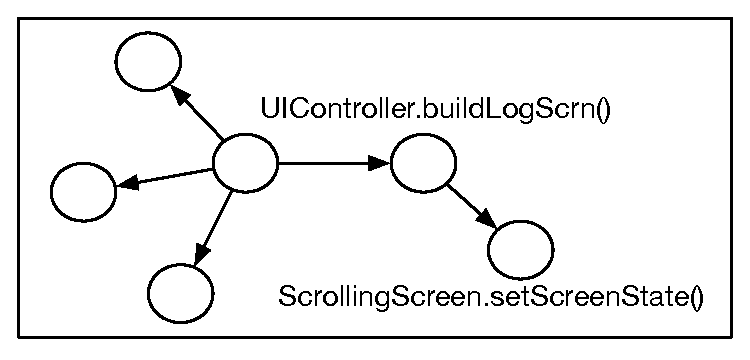
\includegraphics[width=0.8\textwidth]{./figures/example/buildLogScrn.pdf}
    \caption{与日志记录、展示功能有关的部分函数及其依赖结构}
    \label{F:BuildLogScrn}
\end{figure}

我们认为,与变更代码元素在结构上有紧密依赖关系的其他代码元素同样有价值,在这个例子中,函数\emph{setScreenState()}与且只与函数\emph{buildLogScrn()}存在函数调用依赖,因此我们认为这两个函数之间的关系紧密,可能用于实现相似的功能,函数\emph{setScreenState()}的文本信息能够补充与变更有关的概念。在此例中,函数\emph{setScreenState()}包含了有效关键词\ “screen”\ 和\ “state”\ ,这两个概念在\emph{buildLogScrn()}中无法体现,从而补充了与变更有关的概念,达到提高检索精度的目的。

\begin{figure}[thb]
    \centering
    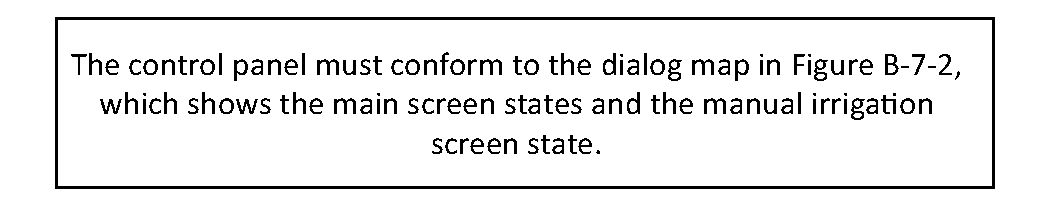
\includegraphics[width=0.8\textwidth]{./figures/example/SRS238.pdf}
    \caption{需求文本SRS238的内容}
    \label{F:SRS238}
\end{figure}

\begin{figure}[thb]
    \centering
    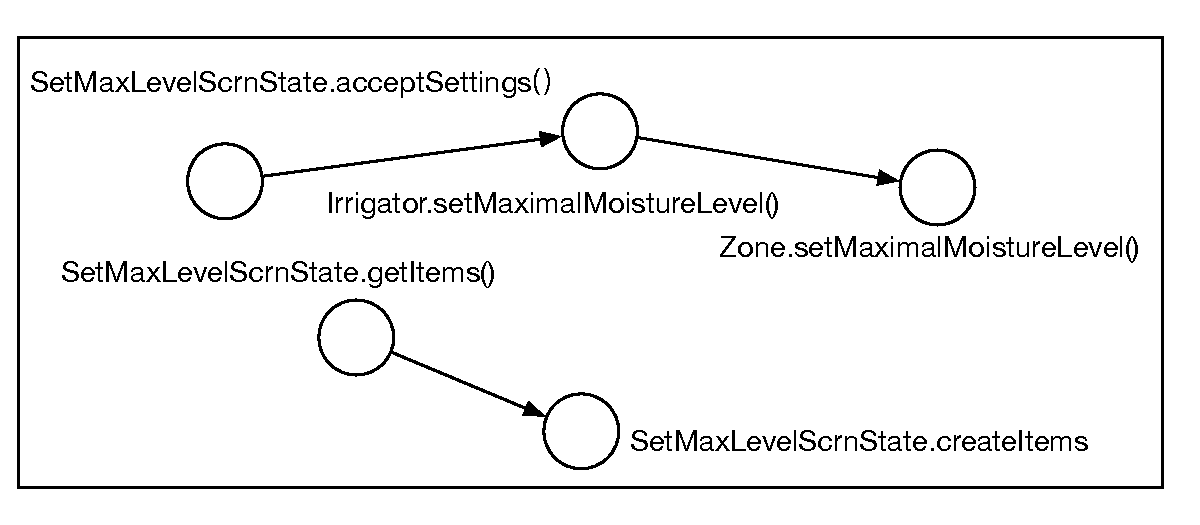
\includegraphics[width=0.8\textwidth]{./figures/example/setMaximalMoistureLevel.pdf}
    \caption{与设置灌溉区域的湿度值上限功能有关的部分函数及其依赖结构}
    \label{F:SRS238}
\end{figure}

在浏览检索结果时,对于特定的某个候选过时需求,维护人员通常需要一些与候选过时需求相关的代码变更情况,从中获取与变更有关的知识,以完成对候选过时需求的更新。例如,维护人员希望获知在此次更新中,哪些关键函数对目标需求构成了影响,维护人员可以根据这些关键函数的行为判断目标需求应该如何更新。图二同样为AquaLush系统中一次真实的代码提交,该提交为AquaLush系统设置了灌溉区域的湿度值上限,图中的函数均为在此次提交中新增的函数。通过观察新增函数的文本信息和结构依赖我们发现,函数\emph{Irrigator.setMaximalMoistureLevel()}与函数\emph{Zone.setMaximalMoistureLevel()}协作完成了此次提交所描述的设置灌溉区域的湿度值上限这一主要行为,应该优先推荐给维护人员作为更新需求的辅助参考。与函数\emph{getItems},\emph{createItems}相比,函数\emph{setMaximalMoistureLevel}既包含与变更有关的重要概念,又此概念在新增函数的调用链上反复出现,因此我们认为具有这样特征的函数应该具有较高的权重,成为维护人员主要关注的函数。


\subsection{问题定义}

\textbf{\emph{问题定义.}} \emph{给定一个需求集合~\emph{R}~,该需求集合包含~d~个需求文本,同时给定新版本代码集合~\emph{NC}~与旧版本代码集合~\emph{OC},分别包含~m~,n~个代码实体(类),过时需求自动检测技术能够从~d~个需求文本中选择~k~个需求文本并排序,作为近似候选过时需求的排序,问题是:}

Q1: 分析代码依赖关系是否能够提高过时需求自动检测方法的精度?

Q2: 对于给定的候选过时需求,能否推荐与该需求更新相关的变更代码元素?

\section{方法概述}

在本节,我们将介绍基于代码依赖关系的过时需求自动检测与更新推荐方法的流程。在维护人员完成代码提交后,我们将给定的新、旧版本代码,需求作为方法的输入,将近似候选过时需求的排序,辅以与候选过时需求相关的变更函数推荐作为输出。方法主要包含三个步骤(1)代码依赖关系构成的代码变更组识别;(2)基于变更组文本与需求文本相似性的过时需求排序生成;(3)基于代码依赖关系与文本信息的变更函数推荐。

\begin{figure}[thb]
    \centering
    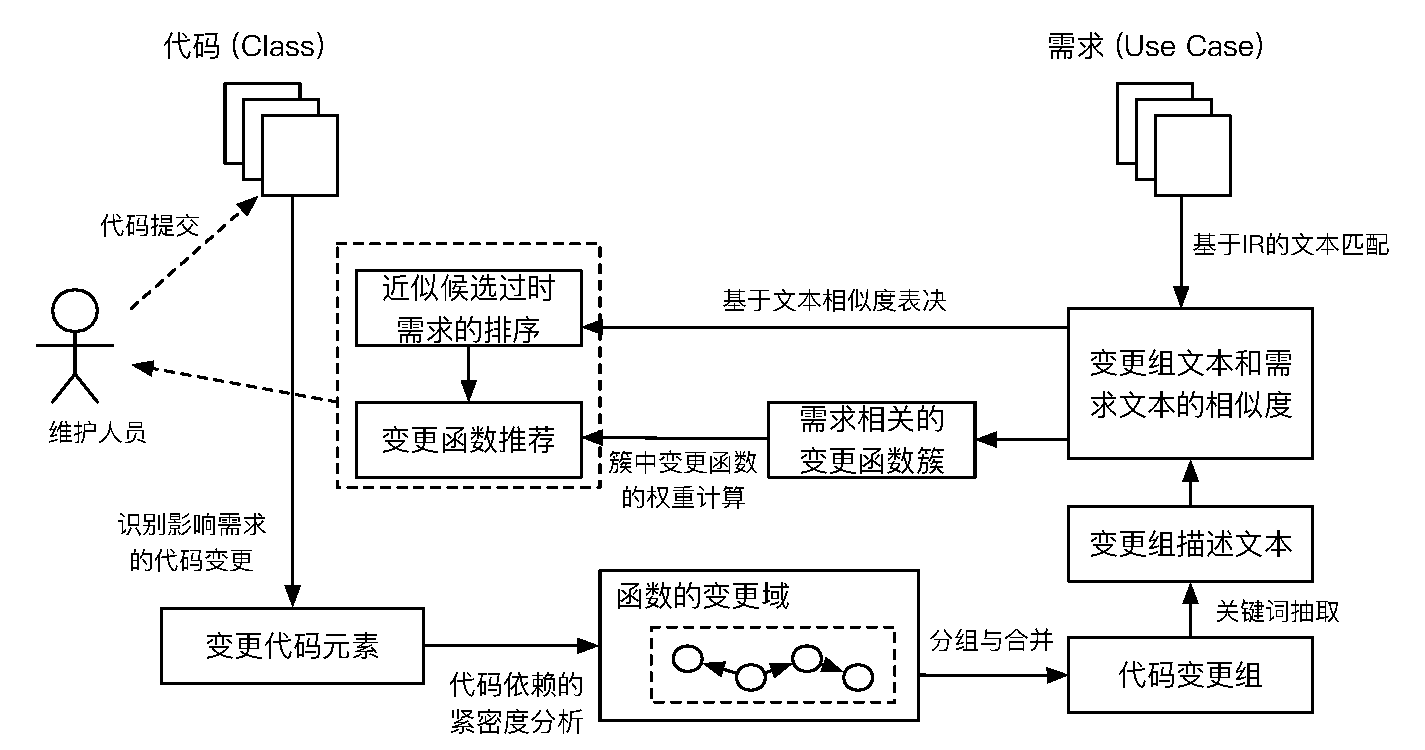
\includegraphics[width=0.8\textwidth]{./figures/approach/approach_overview.pdf}
    \caption{基于代码依赖关系的过时需求自动检测与更新推荐方法流程}
    \label{F:ApproachOverview}
\end{figure}

如图N所示,在步骤一中,方法通过比较代码元素的差异的方式识别出变更代码元素,这些变更代码元素被认为是影响需求的代码变更。然后,基于代码依赖关系的紧密度分析,能够获取与变更函数紧密依赖的其它函数元素,从而建立函数的变更域,并通过变更代码元素的分组与变更域的合并构成代码变更组;在步骤二中,对于每一个代码变更组,我们抽取变更组内代码元素的关键词以构造变更组描述文本,并通过信息检索技术计算变更组描述文本与需求文本的相似度。然后,利用基于相似度值的表决算法生成近似候选过时需求的排序;在步骤三中,对于排序中的候选过时需求,我们能够发现与该需求有关的变更函数,然后根据函数调用依赖将变更函数划分为若干变更函数簇,并基于TF-IDF计算簇中变更函数的权重,从而生成变更函数推荐的排序。在后续章节中,将对上述三个步骤进行详细的阐述。

\section{代码依赖关系构成的代码变更组识别技术}
\subsection{比较代码元素的差异}

在软件演化的过程中,并非所有的代码变更都会影响需求。事实上,其中许多的代码变更与缺陷修复,重构或更改系统实现细节等方面有关。Eya等人[]中提出:代码元素(包,类,函数,域)的新增或删除是影响系统外部行为,从而影响需求的代码变更。文献比较了新旧版本代码间的代码元素,以识别出新增或删除的代码元素,并过滤其中与重命名有关的变更,获得影响需求的变更代码元素。

以变更代码元素为基础,我们假定一个新增的包是有若干新增的类组成,一个新增的类是有若干新增的函数和域组成,对删除的代码元素也进行类似的处理。为描述变更代码元素,给定函数的变更集合$CM = \{CM_{1}, \cdots, CM_{n}\}$, 其中$CM_{i}$为新增或删除的函数,域的变更集合$CF = \{CF_{1}, \cdots, CF_{n}\}$,其中$CF_{i}$为新增或删除的域。

\subsection{构造变更组}
\subsubsection{生成CDCGraph (Call Dependency with Closeness Graph)}
我们利用CDCGraph以描述一个版本源代码中的函数调用依赖及其依赖的紧密度值。我们生成CDCGraph的算法包括以下两个步骤:
\begin{enumerate}
  \item 建立函数的调用依赖:首先,我们定义图CDGraph(Call Dependency Graph)为一个有序对$CDGraph = <V, E>$,其中$V$是代码中函数的集合,$E$是函数间产生的函数调用依赖集合。函数调用依赖是指,如果函数A调用了另一个函数B,那么函数A依赖于函数B。我们利用Apache BCEL库从编译后的字节码(Jar文件)中捕获函数调用依赖,对于无法直接编译的项目,我们基于JDT实现了一个工具,它能够直接从项目的Java源文件中捕获函数的调用依赖。

  \item 计算函数调用依赖的紧密度值:在CDGraph中,函数之间的调用依赖只有存在或不存在两种可能,存在的所有函数调用依赖都被认为是等价的,没有对依赖的紧密程度作出区分。事实上,当函数A调用函数B的时,可能意味着以下两种情况:函数A和函数B通过协作完成某个共同的任务,两者间具有较强的依赖关系;函数A通过调用函数B实现任务间的转移,两者间具有较弱的依赖关系。为了度量函数调用依赖,我们提出紧密度值以量化函数之间的相互作用程度。我们假定,对于函数调用依赖,如果调用者的出度和被调用者的入度越小,则该函数依赖越紧密。我们定义函数调用依赖的紧密度原则的计算公式如下:
  \begin{align}Closeness_{e}=\frac {2} {OutDegree_{e.caller}+InDegree_{e.callee}}\end{align}
  其中,$OutDegree_{e.caller}$表示调用者的出度,$InDegreee.callee$表示调用者的入度。通过赋予CDGraph中的依赖边紧密度值的方式,可得CDCGraph。
\end{enumerate}

\subsubsection{建立函数的变更域}
对于变更的函数元素,我们考虑该元素的结构上下文信息,以补充与变更相关的知识。因此,我们将变更的函数元素及与其结构上紧密依赖的其他函数元素共同构成一个变更域。基于生成的CDCGraph,我们给定一个阈值$k$,将CDCGraph中所有紧密度值小于$k$的依赖边删去。剪枝后的CDCGraph被分解为若干个连通子图,每个连通子图表示一个区域,区域中的函数间被认为具有较强的相互作用程度。我们给定两个函数$\beta$和$\gamma$:第一个函数$\beta \left( CM_{i}\right)$,返回函数CMi在CDCGraph中所属的连通子图;第二个函数$\gamma \left( G_{i}\right)$,返回图$G_{i}$中所包含顶点元素的集合。对于每个变更的函数元素,它对应的变更域可表示为:
\begin{align}
CR_{i}=\gamma\left( \beta \left( CM_{i}\right) \right) 
\end{align}
其中,$CM_{i}$为集合$CM$中一个变更的函数元素。

\subsubsection{分组策略}
对于变更的函数元素,在建立其变更域后,如果孤立地考虑每一个变更域将会导致域的数量过多,并且每个变更域自身的信息可能仍不足以描述一个相对完整的系统功能。因此,我们将基于依赖关系对变更域进行合并。如果集合CM中的函数彼此之间存在函数调用依赖,则合并各个函数对应的变更域,合并后的域我们称之为一个变更组,给定集合$CG = \{CG_{1}, \cdots, CG_{n}\}$以表示变更组的集合,其中$CG_{i}$表示合并后的变更组。另外的,如果变更的函数元素使用了集合$CF$中变更的域元素,则将被使用的域元素加入变更的函数元素所属的变更组。我们定义变更代码元素间的依赖关系图$DG = <V, E>$,其中$V$表示变更代码元素,$E$表示函数调用依赖或域的使用依赖。构造变更组的具体算法如下:

\begin{algorithm}[htbp]
\caption{Change Groups Constructing}
\label{alg:ChangeGroups}
\KwIn{$\emph{DG}$, $\emph{CM}$, $\emph{CF}$, $\emph{CR}$.}
\KwOut{change groups $\emph{CG}$.}
    $CG$ $\leftarrow$ $\emptyset$;\\
    \ForAll {$CM_{i}$ in $CM$}
    {
       \If {isAllocated($CM_{i}$) $= false$}
       {
          methods $M$ $=$ $DG$.getConnectedGraphByCall($CM_{i}$);\\
          elements $e$ $\leftarrow$ $\emptyset$;\\
          \ForAll {$m_{i}$ in $M$}
          {
            ChangeRegion $CR_{i}$ $=$ $CR$.findChangeRegion($m_{i}$);\\
            $e$.add($CR_{i}$);\\
          }
          $CG$.add($e$);\\
          setAllocated($M$);\\
       }
    }

    \ForAll {$CG_{i}$ in $CG$}
    {
       \ForAll {$CM_{i}$ in $CG_{i}$}
       {
          fields $F$ $=$ $DG$.findFieldsUseage($CM_{i}$, $CF$);\\
          $CG_{i}$.add($F$);\\
       }
    }
\end{algorithm}

\section{基于变更组文本与需求文本相似性的过时需求自动检测方法}
\subsection{抽取关键词以构造变更组的描述文本}

在此小节,我们从变更组的代码元素中抽取关键词以构造变更组的描述文本。对于不同来源的代码元素,我们根据规则(见表N)抽取与代码元素相关的标识符,注释等信息,可以注意到,与未变更的代码元素相比,我们会为变更代码元素抽取更多相关的信息。抽词规则确立的依据是,代码元素的标识符和注释信息通常反映了需求中与系统功能相关概念。同时,与未变更的代码元素相比,我们认为变更代码元素与概念的变更有更高的相关性。对于集合$CG$中的每一个变更组$CG_{i}$,通过抽取关键词可以构造变更组描述文本$CGD_{i}$,$CGD_{i} \in CGD$。

\begin{table}[]
\centering
\caption{变更组中代码元素的抽词规则}
\label{my-label}
\begin{tabular}{cccc}
\hline
Element                 & Changed Type  & Identifiers                      & Comments                                                        \\ \hline
\multirow{2}{*}{Method} & Added/Removed & Method, parameters, parent class & \begin{tabular}[c]{@{}c@{}}Method, \\ parent class\end{tabular} \\
                        & Unchanged     & Method, parameters, parent class & No                                                              \\
Field                   & Added/Removed & Field, parent class              & Parent class                                                    \\ \hline
\end{tabular}
\end{table}

\subsection{基于信息检索技术生成近似候选过时需求的排序}
对于给定的变更组文本集合$CGD = \{CGD_{1}, \cdots, CGD_{n}\}$与需求集合$R = \{R_{1}, \cdots, R_{n}\}$,我们通过以下两个步骤生成近似候选过时需求的排序:(1)利用信息检索技术计算变更组文本与需求文本的相似性;(2)利用基于文本相似度值的表决算法,生成近似候选过时需求的排序。我们将在本小节余下部分详细阐述每个步骤。
\begin{enumerate}
  \item 利用信息检索技术的计算文本相似性:基于信息检索的文本匹配技术将两个文本集合作为输入,返回文本-文本的相似度矩阵作为输出。在本方法的场景下,我们计算的是变更组文本与需求文本间的相似性,因此,我们的输入包括变更组文本集合与需求文本集合,预期得到的输出是变更组文本-需求文本的相似度矩阵。 在检索之前,我们需要对变更组文本及需求文本进行预处理。首先,对于词项来自代码的变更组文本,我们根据常用的代码命名模式(如驼峰命名法,下划线分割)进行分词操作。然后,我们对变更组文本和需求文本进行标准化处理,处理的过程包括除去特殊字符,词行还原,词根提取和去停用词。我们利用$tf-idf$[11]计算词项的权重,并利用向量空间模型计算文本相似度。

  \item 基于文本相似度的表决算法:步骤一的结果是一个二维的相似度矩阵,我们基于该矩阵生成一个最终的排序列表,以向维护人员指明潜在的过时需求。我们基于文本相似度值计算最终排序列表的表决算法如下:对于每一个需求文本,累加其与变更组文本集合中各个变更组文本的相似度值,作为该需求的总得分。然后,将需求集合按需求的总得分倒叙排列,作为近似候选过时需求集合的最终排序,需求的排名越高代表该需求是过时需求的可能性越大。
\end{enumerate}

\section{基于代码依赖关系与文本信息的过时需求半自动更新推荐机制}
在维护人员浏览近似候选过时需求的排序时,对于给定的某个候选过时需求,基于代码依赖关系与文本信息的过时需求半自动更新推荐机制能够推荐相关的变更代码元素,以辅助维护人员完成对过时需求的更新。通常情况下,函数是用于表达系统某个功能实现的基本粒度。因此,本方法主要关注于对变更函数的推荐。

首先,对于给定的候选过时需求,我们基于4.x.y中的变更组文本-需求文本相似度矩阵以发现与该需求有相似性的变更组(两者的相似度值大于零),这些变更组所包含的变更函数构成候选变更函数集合$CCM = \{CCM_{1}, \cdots, CCM_{n}\}$。然后,我们将集合$CCM$中的变更函数根据权重排序以推荐给维护人员。变更函数的排序过程分为以下两个步骤:
\begin{enumerate}
  \item 基于代码依赖关系构造变更函数簇:利用4.x.x中变更代码元素间的依赖关系图DG,我们将变更函数根据函数调用依赖划分为若干变更函数簇,其中每个变更函数簇是一个连通的函数调用依赖图,我们用集合$CMC$表示变更函数簇的集合,其中$CMC_{i}$由变更函数构成。
  \item 基于TF-IDF的变更函数权重计算:
  我们假定变更函数的权重是基于变更函数(标识符)中所包含词的权重计算而得。因此,我们首先根据代码的文本信息计算变更函数中词的权重。我们采用TF-IDF加权技术以评估词的重要性,我们同时考虑词对于变更函数簇的重要性(局部重要性)和词对于代码库的重要性(全局重要性)。我们认为,如果某个词在变更函数簇中出现的频率高,并且在代码库中很少出现,则认为此词与变更概念具有较高的相关性,包含该词的变更函数适合推荐给维护人员,以提供与变更概念有关的知识。

  为此,我们首先构造变更函数簇文本集和代码库文本集。对于每一个变更函数簇,我们抽取簇中变更函数的标识符(包括函数名,及函数所属类的类名)构成变更函数簇文本。同时,我们提取更新前代码库中的所有函数,每个函数作为一个文本,文本内容同样为函数的标识符。然后,利用构造的变更函数簇文本集和代码库文本集,基于TF-IDF计算变更函数簇中词的权重。TF-IDF的计算公式如下:
  \begin{align}
    tf_{i,j}=\dfrac {n_{i,j}} {\sum _{k}n_{k,j}}
  \end{align}
  \begin{align}
    idf_{i}=\log \dfrac {\left| D\right| } {\left| j:t_{i}\in d_{j}\right| }
  \end{align}
  \begin{align}
    tfidf_{i,j}=tf_{i,j} \times idf_{i}
  \end{align}
  其中,$tf$指给定的某一个词在文本中的出现频率。$n_{i,j}$为词$t_{i}$在文本$d_{j}$中的出现次数,分母表示在文本$d_{j}$中所有词的出现次数之和;$idf$(inverse document frequency)用于度量词的普遍重要性,$\left| D\right|$表示语料库中的文本总数,表示包含词$t_{i}$的文本数目。在本方法的场景中,$d_{j}$对应变更函数簇文本,语料库$D$包括变更函数簇文本和从代码库中提取的函数文本。最终,变更函数的权重由该函数标识符所包含词权重的算术平均确定,其中词的权重为该词在此变更函数所属的变更函数簇文本中的权重。我们将集合$CCM$中的变更函数根据权重倒叙排列,作为变更函数推荐的排序。
\end{enumerate}







\section{实验与分析}

在此小节,我们通过实验以验证本方法的有效性。接下来,将具体阐述我们的实验设置及实验结果与分析。

\subsection{实验目标与评价指标}
我们的实验目的是为了分析基于代码依赖关系的过时需求自动检测方法是否能够减少维护人员发现过时需求的成本。为了达到这一目的,我们需要回答4.2.1中定义的如下两个研究问题。

Q1: 分析代码依赖关系是否能够提高过时需求自动检测方法的精度?

这个研究问题与我们方法的第一部分有关,在x.x节中,我们验证了基于代码依赖关系的过时需求自动检测方法的有效性。

Q1的评价指标:Q1是关于从整个需求集合里检测某一特定的子集(过时需求),因此我们采用信息检索中著名的两个指标$Average \  Precision\left( AP\right)$和$F-measure$以评价近似候选过时需求排序的质量。
\begin{align}
AP=\dfrac {\sum _{r=1}^{N}\left( Precision\left( r\right) \times isRelevant\left( r\right) \right) } {\left| RelevantDocuments\right| }
\end{align}

其中,$r$表示目标文本在有序文本列表中的排序,$Precision\left( r\right)$表示前$r$个排序的准确率,$isRelevant\left(\right)$是一个二值函数,如果文本相关返回1,无关则返回0,$N$表示文本的总数。同时,$F-measure$是准确率和召回率的调和平均值,计算方式如下:
\begin{align}
F=\dfrac {2} {\dfrac {1} {R}+\dfrac {1} {P}}\end{align}

其中,R表示召回率,P表示准确率。我们通过统计显著性检验以验证我们方法能够在不同的截止排序n上提高其$F-measure$值。由于过时需求的总数对于每个检测方法是一致的,因此我们采用Wilcoxon秩和检验[]以检验如下的两个零假设(null hypothesis):

$H_{0}$:在代码提交版本间,分析代码依赖关系没有显著的提高过时需求需求自动检测方法的精度。

$H_{1}$:在代码发布版本间,分析代码依赖关系没有显著的提高过时需求需求自动检测方法的精度。

我们采用$p-value$显著性差异水平0.05作为衡量检验结果的标准。除了$p-value$以外,我们关注的另一方面是在实践中不同方法精度间的差异幅度。为此,我们采用$Cliff’s \ Delta \ d$[68],一种应用于序数的无参效果量($effective \ size$)来衡量实验组与对照组的差异($p-value$表明显著性是否存在,$effective \ size$表明实践的显著程度)。$Cliff’s \ Delta$的范围在-1和1之间,$d\ \textless \ 0.33$表示显著性较小,$0.33\ \leq \ d \ \textless \ 0.474$表示显著性一般,$d\ \geq \ 0.474$表示显著性较大。

Q2: 对于给定的候选过时需求,能否推荐与该需求更新相关的变更代码元素?

这个研究问题与我们方法的第二部分有关,在x.x.x节中,我们验证了基于代码依赖关系和文本信息的变更函数推荐方法的有效性。

Q2的评价指标:Q2是关于从所有变更函数里选取某一特定的子集,并将选取的变更函数按权重排序推荐给维护人员,通常推荐排序中的每一项(变更函数)会根据其与需求更新的相关程度而被打分。因此我们采用两个衡量排序质量的指标$DCG$(Discounted cumulative gain)和$NDCG$(Normalized Discounted cumulative gain)用以评价我们的方法。使用DCG指标时有两个基本假设条件:(1)在排序列表中,相关性越高的结果排序越靠前越有益。(2)在对排序列表中的每一项标注时,评分等级高的结果比等级低的结果有益。我们的评价场景符合上述两个基本假设条件。$DCG$的核心思想是如果评分等级较高的项却排序较后,那么在计算排序的得分时就需要对该项的得分有所惩罚,DCG的公式如下:
\begin{align}
DCG_{p}=rel_{1}+ \sum _{i=2}^{p}\dfrac {rel_{i}} {\log _{2}\left( i\right) }
\end{align}

其中$rel_{i}$表示排序为i项的评分。为了便于不同类型查询所得到的结果之间横向比较,并衡量当前排序与理想排序的差异,$NDCG$通过将当前结果排序的DCG值除以该查询结果的理想值$IDCG$(Ideal DCG)的方式进行归一,公式为:
\begin{align}
NDCG_{p}=\dfrac {DCG_{p}} {IDCG_{p}}
\end{align}
在实际中,标定$IDCG$值的操作较为困难,我们在4.4.4节中给出了标定变更函数推荐排序$IDCG$值的方式。


\subsection{研究案例与实验设置}

\begin{enumerate}
  \item iTrust

  我们第一个研究案例是医疗服务项目iTrust[16],iTrust是一个医疗数据管理系统,它是由北卡罗莱纳州立大学开发并维护的一个用于教学目的的系统。iTrust包含多个发布的代码版本和一个基于wiki的规约说明,规约说明中包括功能性需求,非功能性需求,术语表等信息。iTrust是由Java和Java Server Page组合开发的Web应用。在我们的实验中,需求部分我们选用iTrust中的39个功能性需求,每个功能性需求是详细且定义良好的用例(use case)。在代码部分,由于我们的原型工具暂时只支持对Java代码的分析,因此我们只考虑iTrust中Java部分的源码。我们使用iTrust版本10(发布日期:2010.8.18)和版本11(发布日期:2011.1.7)作为两个发布的代码版本。Eya在文献[]中通过人工比较这两个版本源代码的方式,发现了14个概念变更,并识别了这些变更所影响的需求。我们选取了其中10个影响需求的变更作为代码提交。

  表N中展示了我们验证Q1时所选取的代码变更,变更的描述,以及变更所影响的需求。同时,为了验证Q2,对于在一次变更中特定的某个过时需求,我们将除去过时需求包含语料后的变更的描述作为变更概念的文本,计算推荐的变更函数标识符中,命中变更概念文本中词的准确率,作为该变更函数的评分。根据变更函数的评分,可以计算推荐变更函数排序的DCG值。将变更函数按评分倒叙排列,可以得到变更函数推荐的理想排序,并标定$IDCG$值。由于iTrust中代码提交的描述信息较少,存在变更函数排序中的函数无法命中变更概念文本中词的情况,因此在实验中我们并不比较此类代码提交。

  \begin{table}[]
  \centering
  \caption{iTrust系统中的代码变更及变更所影响的需求}
  \label{my-label}
  \begin{tabular}{@{}lll@{}}
  \toprule
  Change & Change description                             & Impacted use cases \\ \midrule
  Change 1          & Reason code                                    & UC15, UC37         \\
  Change 2          & Uploading photo                                & UC4                \\
  Change 3          & Remote monitoring (added height, weight, etc.) & UC34               \\
  Change 4          & Remote monitoring (get patient data by type)   & UC34               \\
  Change 5          & Display patient’s monitoring HCP               & UC34               \\
  Change 6          & Office visit form (added orc and comment)      & UC11               \\
  Change 7          & Enabling appointment editing                   & UC22               \\
  Change 8          & Login (added captcha and attempts)             & UC3                \\
  Change 9          & Weight/height charting                         & UC10               \\
  Change 10         & Logging (added logs)                           & UC5                \\ \bottomrule
  \end{tabular}
  \end{table}

  \item AquaLush

  我们第二个研究案例是由软件控制的灌溉管理系统[],可以基于用户提供的湿度、用水量等参数自动调整灌溉输出,AquaLush最初作为一个解释性示例在《软件设计导论》[14]一书中被提出。AquaLush由Java语言实现,代码量在1.1万行左右,同时,AquaLush包含自然语言描述的结构化需求规约。网页[]包含AquaLush的代码,需求和基线等相关。在需求的部分,我们的实验提取了需求规约中文本格式的337个需求说明作为需求规约集合;在代码的部分,Eya在文献[]中开发了AquaLush的另一个版本,相比原版本,新版本包含了8次代码提交(3次与系统功能有关和5次与缺陷修复有关)。我们选取了3次与系统功能有关的代码提交,并将上述两个版本作为两个代码的发布版本。表N中展示了我们验证Q1时所选取的代码变更,变更的描述,以及变更所影响的需求。我们同样采取计算推荐的变更函数标识符中,命中变更概念文本中词的准确率作为变更函数的评分以验证Q2。

% Please add the following required packages to your document preamble:
% \usepackage{booktabs}
\begin{table}[]
\centering
\caption{AquaLush系统中的代码变更及变更所影响的需求}
\label{my-label}
\begin{tabular}{@{}lll@{}}
\toprule
Change   & Change description                                                                                                                                                                                                                                                                                              & Impacted use cases                                                                                     \\ \midrule
Change 1 & \begin{tabular}[c]{@{}l@{}}Add a maximum moisture level: the irrigation \\ should start when the moisture level is lower \\ than the critical moisture level and should\\ stop as soon as the maximal moisture level is \\ reached. The default max level should be 50.\end{tabular}                            & \begin{tabular}[c]{@{}l@{}}SRS25, SRS26\\ SRS28, SRS53\\ SRS69, SRS359\end{tabular}                    \\
Change 2 & \begin{tabular}[c]{@{}l@{}}Allow setting the water allocation for \\ each of the zones separately\end{tabular}                                                                                                                                                                                                  & \begin{tabular}[c]{@{}l@{}}SRS29, SRS53\\ SRS153, SRS186\\ SRS32, SRS378\\ SRS379, SRS382\end{tabular} \\
Change 3 & \begin{tabular}[c]{@{}l@{}}Create a log that includes the timestamp \\ for each of the following events: change \\ irrigation mode, setting water allocation, \\ setting irrigation time, setting critical, or \\ maximum moisture level. A button show \\ log allows the user the access the log.\end{tabular} & \begin{tabular}[c]{@{}l@{}}SRS238, SRS262\\ SRS266\end{tabular}                                        \\ \bottomrule
\end{tabular}
\end{table}

  \item Connect

  我们第三个研究案例是用于医疗机构间交换医疗数据的开源系统Connect[]。Connect项目包含大量相关的文档,如设计文档,使用手册,问题追踪,变更请求,发布记录,各代码版本的需求,需求跟踪矩阵等。Connect由Java语言实现,并包含历史提交信息。在本实验中,我们采用了主项目部分的Java代码,它位于代码仓库的product/production目录下,代码量在28万行左右。在需求的部分,Eya在文献[]中采用了需求跟踪矩阵及发布记录中Jira单号,其中需求跟踪矩阵关联了需求与Jira问题单号的关系,通过它们之间的关联,发现与相应需求有关的26次代码提交,我们我们选取了其中11个影响需求的代码提交。我们选取了由于Connect中没有提供明确的变更描述,因此我们在验证Q2时,只选用了iTrust和AquaLush系统。
\end{enumerate}

\subsection{实验结果与结果分析}

在本节中,以两个研究问题为指导,我们阐述了三个研究案例的实验结果并给予分析。

\subsubsection{过时需求检测(Q1)}
为了回答Q1,我们在函数调用依赖的紧密度阈值$k=0.3$下进行了实验。我们检验了在前$n$个排序时的$AP$和$F-Measure$值,图N的$F-Measure/Cut$曲线展示了选取前1至30个排序时,代码提交版本间三个研究案例的$F-Measure$,其中红线为基线方法,蓝线。图N为代码发布版本间的$F-Measure/Cut$曲线。表N展示了$AP$与$Wilcoxon$秩和检验结果。

\begin{table}[]
\centering
\caption{平均正确率与Wilcoxon秩和检验结果}
\label{my-label}
\begin{tabular}{@{}ccccc@{}}
\toprule
System                    & Version  & Average Precision & p-value        & Cliff’s Delta     \\ \midrule
\multirow{2}{*}{iTrust}   & commits  & 25.13\% (+20.00\%) & \textless \textbf{\ 0.01} & 0.49 (large)      \\
                          & releases & 66.55\% (+31.87\%) & \textless \textbf{\ 0.01} & 0.73 (large)      \\
\multirow{2}{*}{AquaLush} & commits  & 22.76\% (+4.68\%) & \textbf{\ 0.05}           & 0.29 (small)      \\
                          & releases & 27.65\% (+1.58\%) & \textless \textbf{\ 0.01} & 0.46 (medium)     \\
\multirow{2}{*}{Connect}  & commits  & 42.06\% (+9.29\%) & \textbf{\ 1}              & 0.11 (negligible) \\
                          & releases & 23.04\% (+2.30\%) & \textbf{\ 0.02}           & 0.36 (medium)     \\ \cmidrule(l){1-5} 
\end{tabular}
\end{table}

iTrust:在比较代码提交版本间的过时需求检测结果时,10个代码提交中的5个(Change3,4,5,8,9)在两者方法下都能取得100\%的$AP$值,故我们主要关注在剩余的5个代码提交中,两者方法的表现。如图N中的$iTrust_{Commit}$所示,我们方法的$F-Measure/Cut$曲线能够明显覆盖基线方法的曲线,并且$AP$值从5.57\%提升至25.13\%(提升约20\%,见图N)。$F-Measure/Cut$曲线与基线相比,$p-value < 0.01$,故拒绝零假设$H_{0}$,表明分析代码依赖关系能够明显提高过时需求自动检测方法的精度,在$Cliff’s Delta$下为高效果量。对于代码发布版本间的过时需求检测结果的比较,我们方法的$F-Measure$值仍能够明显覆盖基线方法,并且$AP$值从34.68\%提升至66.55\%(提升约31.87\%,见图N),$p-value<0.01$,故拒绝零假设$H_{1}$,在$Cliff’s Delta$下为高效果量。因此对于iTrust系统,分析代码依赖关系能够明显提高过时需求自动检测方法的精度。

\begin{figure*}[t]
   \subfigure[ $iTrust_{Commits}$ ]{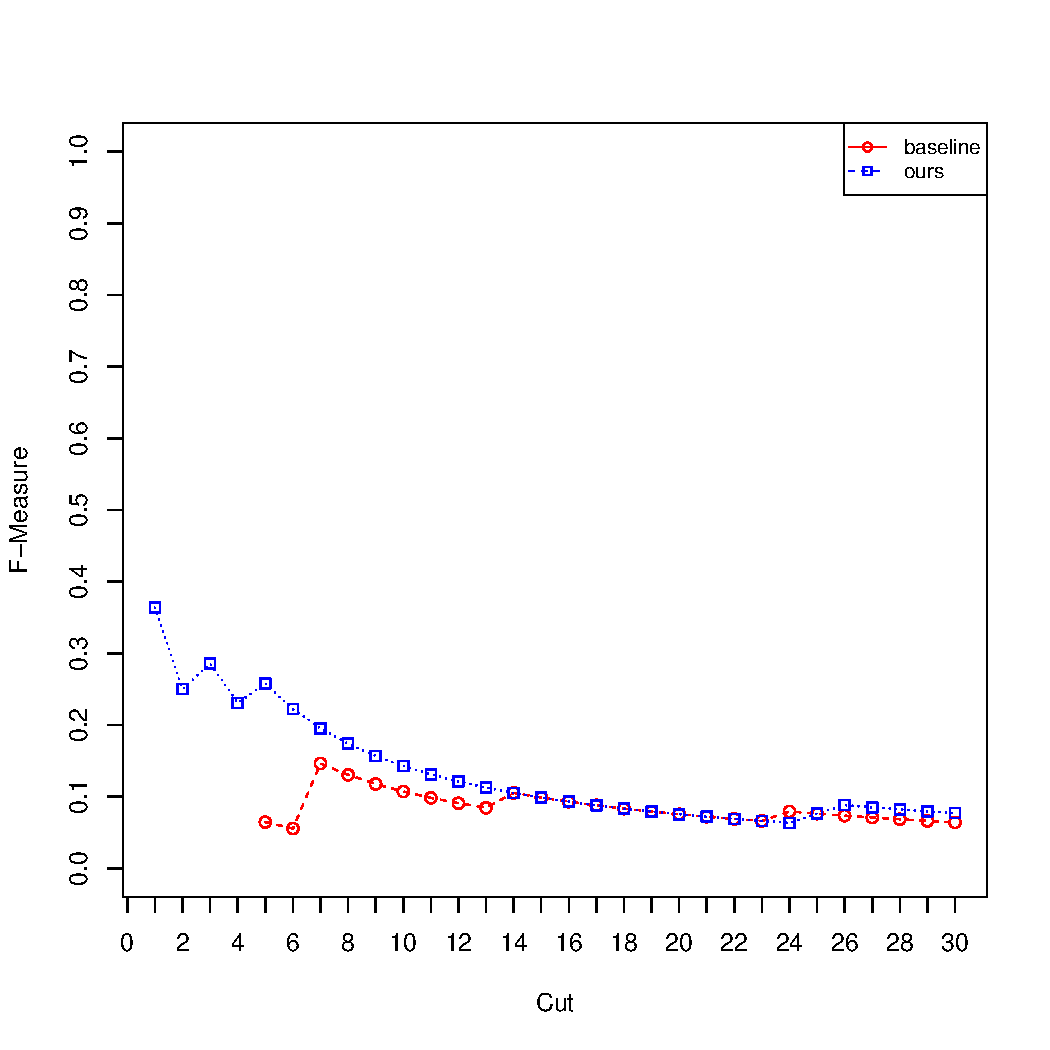
\includegraphics[width=0.31\textwidth,height=0.22\textheight]{figures/iTrust_Commits@30.pdf}
   }
   \subfigure[ $AquaLush_{Commits}$ ]{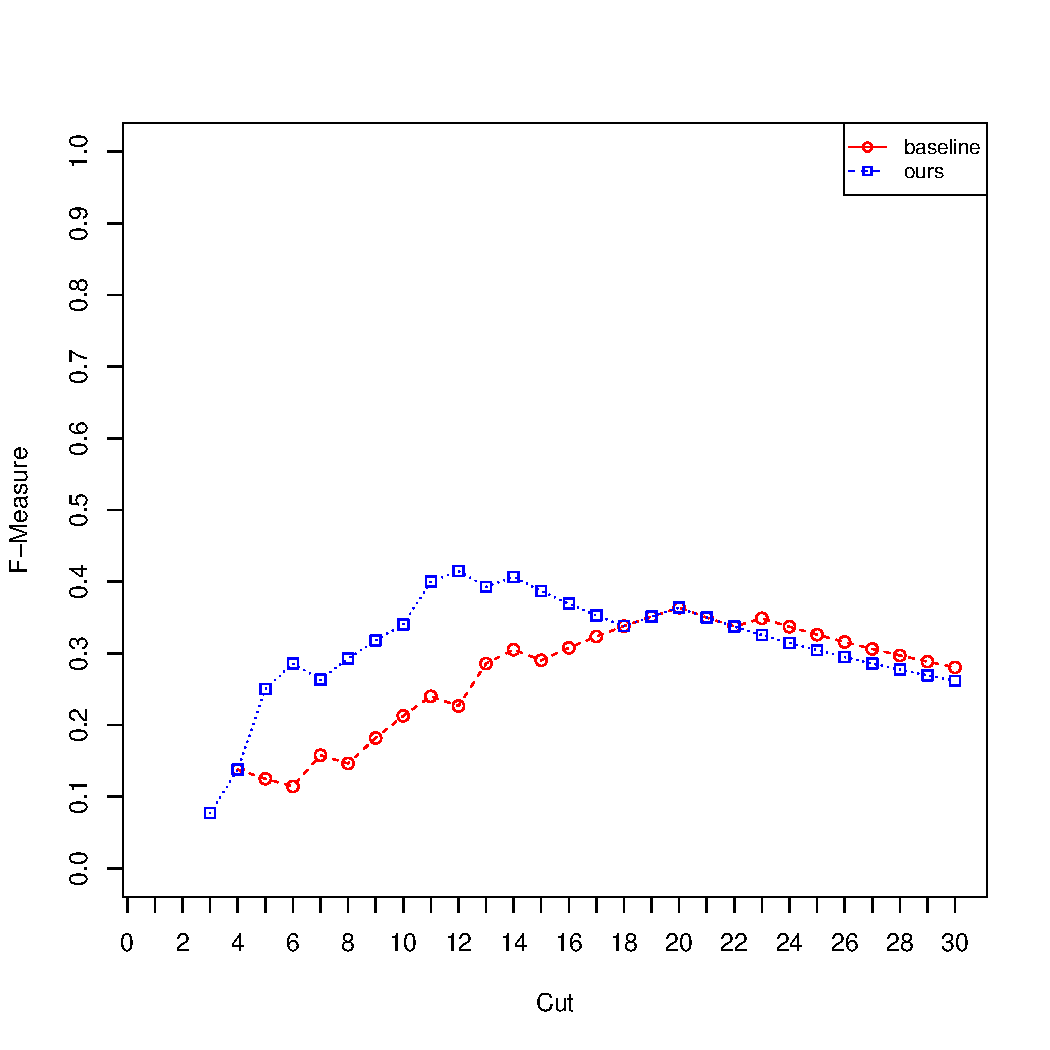
\includegraphics[width=0.31\textwidth,height=0.22\textheight]{figures/Aqualush_Commits@30.pdf}
   }
   \subfigure[ $Connect_{Commits}$ ]{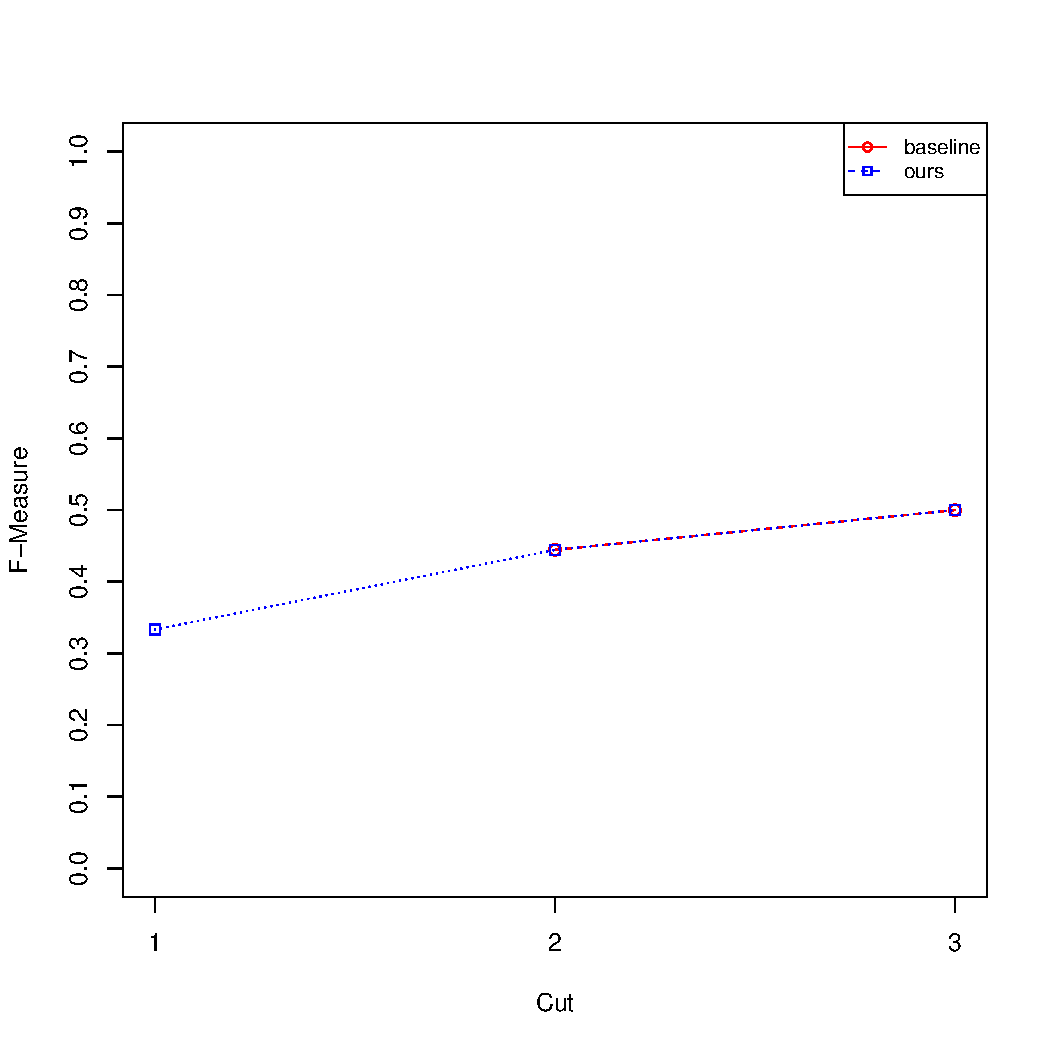
\includegraphics[width=0.31\textwidth,height=0.22\textheight]{figures/Connect_Commits.pdf}
   }
   \caption{F-measure/cut curves for iTrust, AquaLush and Connect between Commits.}
   \label{fmeasure_commits}
\end{figure*}


\begin{figure*}[t]
   \subfigure[ $iTrust_{Releases}$ ]{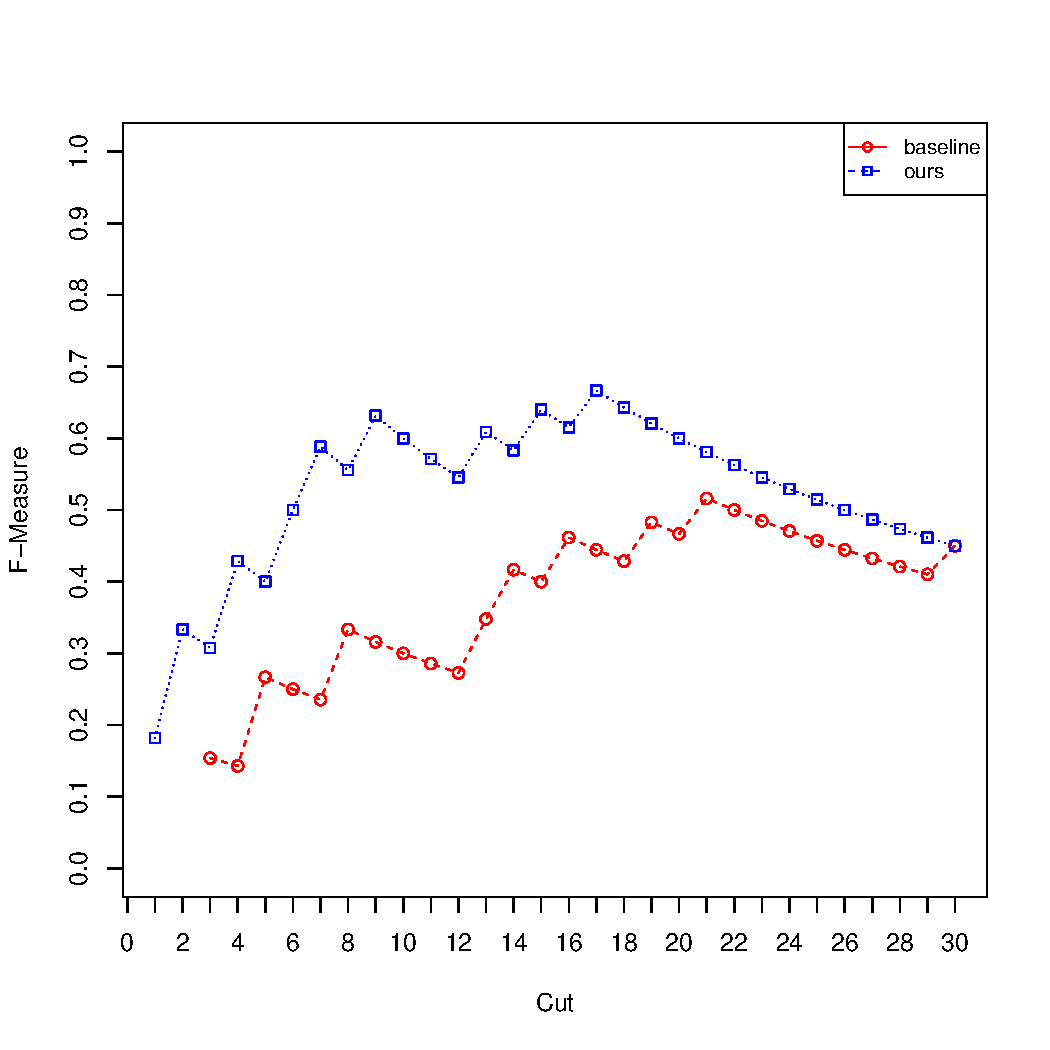
\includegraphics[width=0.31\textwidth,height=0.22\textheight]{figures/iTrust_Releases@30.pdf}
   }
   \subfigure[ $AquaLush_{Releases}$ ]{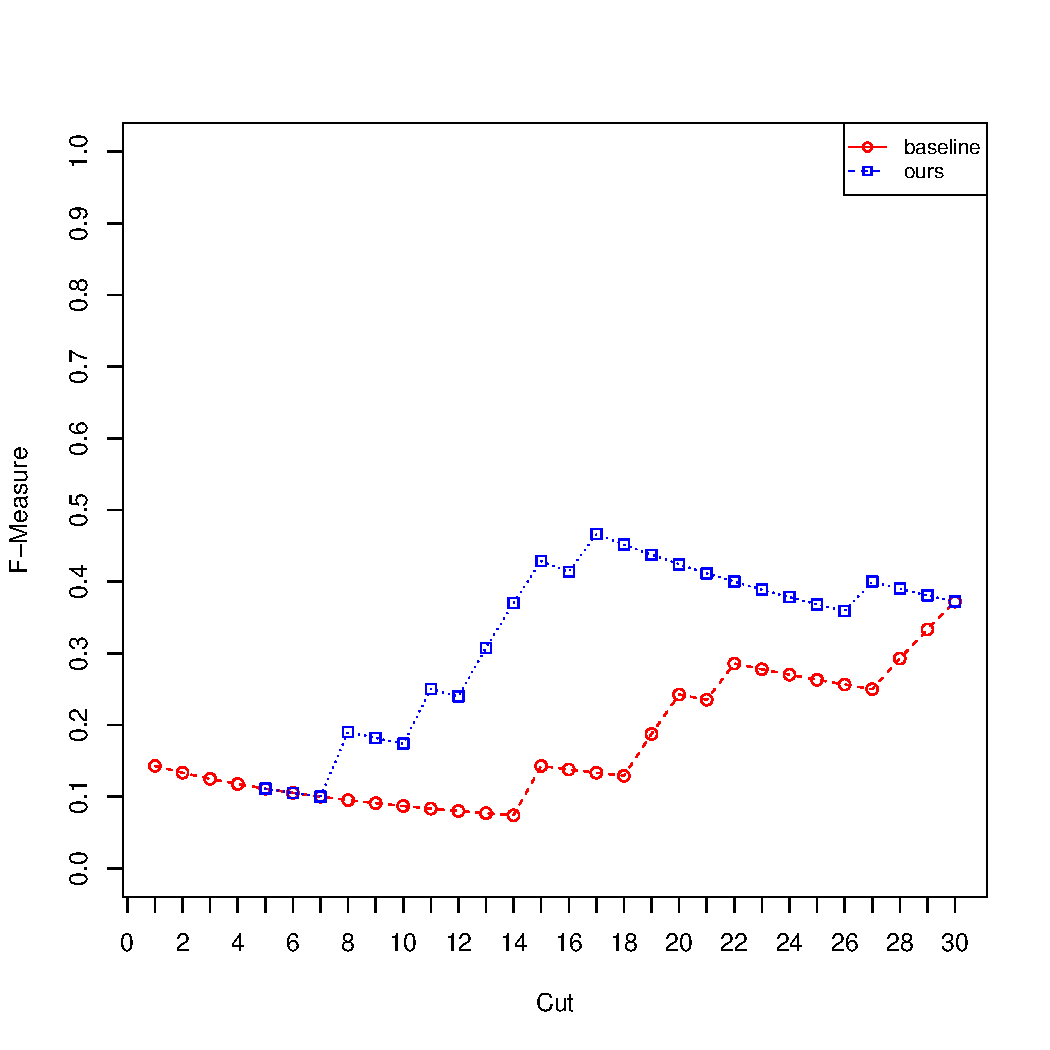
\includegraphics[width=0.31\textwidth,height=0.22\textheight]{figures/Aqualush_Releases@30.pdf}
   }
   \subfigure[ $Connect_{Releases}$ ]{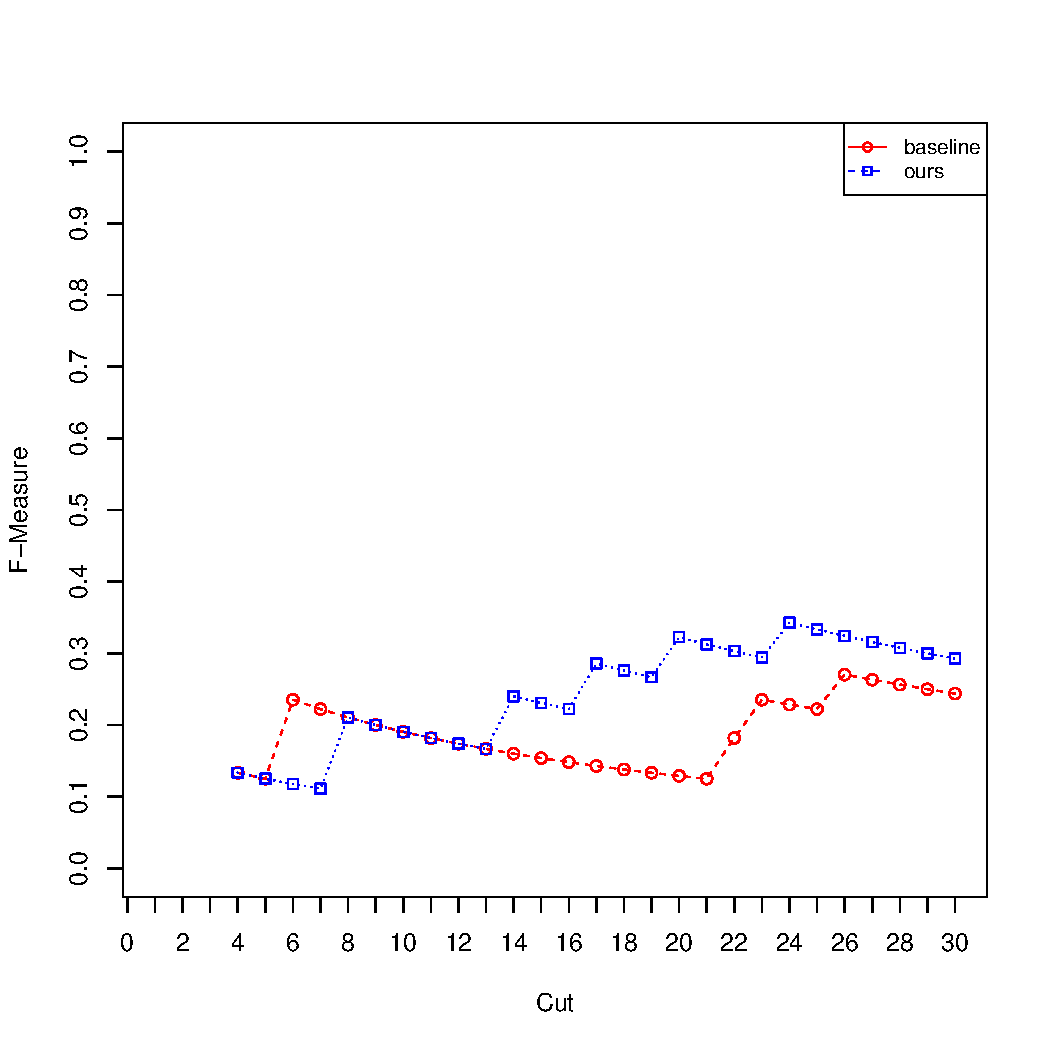
\includegraphics[width=0.31\textwidth,height=0.22\textheight]{figures/Connect_Releases@30.pdf}
   }
   \caption{F-measure/cut curves for iTrust, AquaLush and Connect between Release.}
   \label{fmeasure_release}
\end{figure*}

AquaLush:在比较代码提交版本和代码发布版本的过时需求检测结果时,我们方法的$F-Measure/Cut$曲线值能够明显覆盖基线方法的曲线,$AP$值分别提高了4.68\%和1.58\%,$p-value$值均$<=0$.05,故拒绝零假设$H_{0}$,$H_{1}$。对于AquaLush系统,分析代码依赖关系也能够提高过时需求自动检测方法的精度。

Connect:在比较代码提交版本间的过时需求检测结果时,11个代码提交中的8个在两者方法下都能取得100\%的$AP$值,故我们主要关注在剩余的3个代码提交中,两者方法的表现。如图N中的$Connect_{Commit}$所示,这3个代码提交能够在前3个排序检测出所有的过时需求,$AP$值从32.78\%提升至42.06\%(提升约9.29\%),由于$p-value > 0.05$,因此无法拒绝零假设$H_{0}$。其主要的原因在于,与Connect的三个代码提交有关的过时需求数量较少,且基线方法已经能够较为准确地检测出所有过时需求(过时需求均在前3排序内被发现),因此该实验环境下我们的方法对检测效果的提升空间非常有限。尽管如此,我们的方法在检测时仍然将与代码提交Change841有关的过时需求GATEWAY-841提高了一个排名(从第2提升至第1)。对于代码发布版本间的过时需求检测结果的比较,我们方法的$F-Measure$值在大部分情况下能够明显覆盖基线方法,并且$AP$值从20.74\%提升至23.04\%(提升约2.3\%,见图N),$p-value<0.01$,故拒绝零假设$H_{1}$,在$Cliff’s Delta$下为中效果量。因此对于Connect系统,分析代码依赖关系能够明显提高代码发布版本间过时需求自动检测方法的精度。

结合上述三个研究案例的结果与分析发现,我们的方法提高了近似候选过时需求排序的AP与F-Measure,并通过了6个显著性测试中的5个,可以认为基于代码依赖关系的分析能够显著提高过时需求自动检测的精度。

\subsubsection{变更函数推荐(Q2)}

为了回答Q2,对于与某一次代码提交相关的过时需求,我们检验了前10个推荐的变更函数排序的$DCG$与$NDCG$值。图N展示了iTrust与AquaLush这两个研究案例中各个代码提交下,对于不同过时需求的变更函数推荐排序的平均$DCG$与$NDCG$值,并与传统的字母表排序进行了比较。在计算变更函数推荐排序的$DCG$与$NDCG$
前,我们首先需要为排序中的变更函数标定评分(评分标定过程详见x.x.x节),将变更函数按评分倒叙排列,可以得到变更函数推荐的理想排序及$IDCG$值。

AquaLush: 在与字母表排序的比较中,对于Change1,我们的方法将NDCG值从0.77提升至0.81(提升约0.04,见图N)。对于Change2,我们的方法将NDCG值从0.22提升至0.76(提升约0.54)。对于Change3,我们方法的NDCG值下降了0.03,通过分析发现,这与Change3中变更函数的命名方式和变更描述的质量有关。Change3中的变更函数,如getItems,createItems,getEvent等包含的语义概念较为普遍,缺少独特性,表达的是与底层实现相关的细节概念,而变更描述文本更多的是在阐述与功能相关的概念,两者由于表达层次的不同,存在词汇失配的问题(Vocabulary Mismatch),此时我们用于标定变更函数评分的方式无法准确评价变更函数的重要性,从而影响评价指标的效果。

% Please add the following required packages to your document preamble:
% \usepackage{multirow}
\begin{table}[]
\centering
\caption{AquaLush变更函数推荐排序的DCG与NDCG值}
\label{my-label}
\begin{tabular}{lllll}
\hline
Project                   & Change                   & Rank     & DCG  & NDCG \\ \hline
\multirow{6}{*}{AquaLush} & \multirow{2}{*}{Change1} & Alphabet & 0.66 & 0.77 \\
                          &                          & Ours     & 0.68 & 0.81 \\
                          & \multirow{2}{*}{Change2} & Alphabet & 0.12 & 0.22 \\
                          &                          & Ours     & 0.39 & 0.76 \\
                          & \multirow{2}{*}{Change3} & Alphabet & 1.18 & 0.87 \\
                          &                          & Ours     & 1.09 & 0.80 \\ \hline
\end{tabular}
\end{table}


\begin{table}[]
\centering
\caption{iTrust变更函数推荐排序的DCG与NDCG值}
\label{my-label}
\begin{tabular}{lllll}
\hline
Project                  & Change                   & Rank     & DCG  & NDCG \\ \hline
\multirow{14}{*}{iTrust} & \multirow{2}{*}{Change1} & Alphabet & 1.33 & 0.66 \\
                         &                          & Ours     & 1.33 & 0.72 \\
                         & \multirow{2}{*}{Change2} & Alphabet & 0.93 & 0.75 \\
                         &                          & Ours     & 1.11 & 0.90 \\
                         & \multirow{2}{*}{Change3} & Alphabet & 0.33 & 0.35 \\
                         &                          & Ours     & 0.68 & 0.73 \\
                         & \multirow{2}{*}{Change6} & Alphabet & 0.25 & 0.63 \\
                         &                          & Ours     & 0.37 & 0.94 \\
                         & \multirow{2}{*}{Change7} & Alphabet & 0.82 & 0.85 \\
                         &                          & Ours     & 0.78 & 0.81 \\
                         & \multirow{2}{*}{Change8} & Alphabet & 0.80 & 0.78 \\
                         &                          & Ours     & 0.98 & 0.96 \\
                         & \multirow{2}{*}{Change10} & Alphabet & 0.44 & 0.76 \\
                         &                          & Ours     & 0.58 & 1.0 \\ \hline
\end{tabular}
\end{table}

iTrust:在与字母表排序的比较中,我们的方法在多数情况下(5/7)能够提高变更函数排序的NDCG值(提高0.06~0.37),如图N所示。

结合上述两个研究案例的结果与分析发现,对于给定的过时需求,我们的方法能够推荐与该需求更新相关的变更函数,且在大多数实验结果中(8/10),变更函数推荐的排序比字母表排序有更高的质量。

\section{本章小结}

在本章中,我们提出一种基于代码依赖关系的过时需求自动检测方法,提高了过时需求检测时的精度,并推荐与过时需求更新相关的变更代码元素,以辅助维护人员完成对需求的更新。最后,我们在三个研究案例下设计并完成实验,验证了我们方法的有效性。


\chapter{过时需求自动检测工具实现}

目前,针对过时需求自动检测问题,领域内还没有面向维护人员实际工具。在本章中,我们介绍了过时需求自动检测工具INFORM(IdeNtiFy Outdated RequireMents)的实现,INFORM集成了我们基于代码依赖关系的过时需求自动检测与更新推荐方法,并提供Console与GUI的版本。此外,INFORM的Console版本中集成了代码托管与版本控制服务GitHub的接口,使维护人员在向GitHub进行代码提交后,能够便利地获取潜在的过时需求,降低了需求更新参与一般维护过程的成本。

\section{系统体系结构}

图N展示了INFORM的系统体系结构,其中主要包括用户交互、代码版本比较,代码依赖静态分析,变更组构造及文本抽取,检索与推荐五大模块。在本小节中,我们将对上述五个模块的设计与实现进行说明。

\begin{figure}[thb]
    \centering
    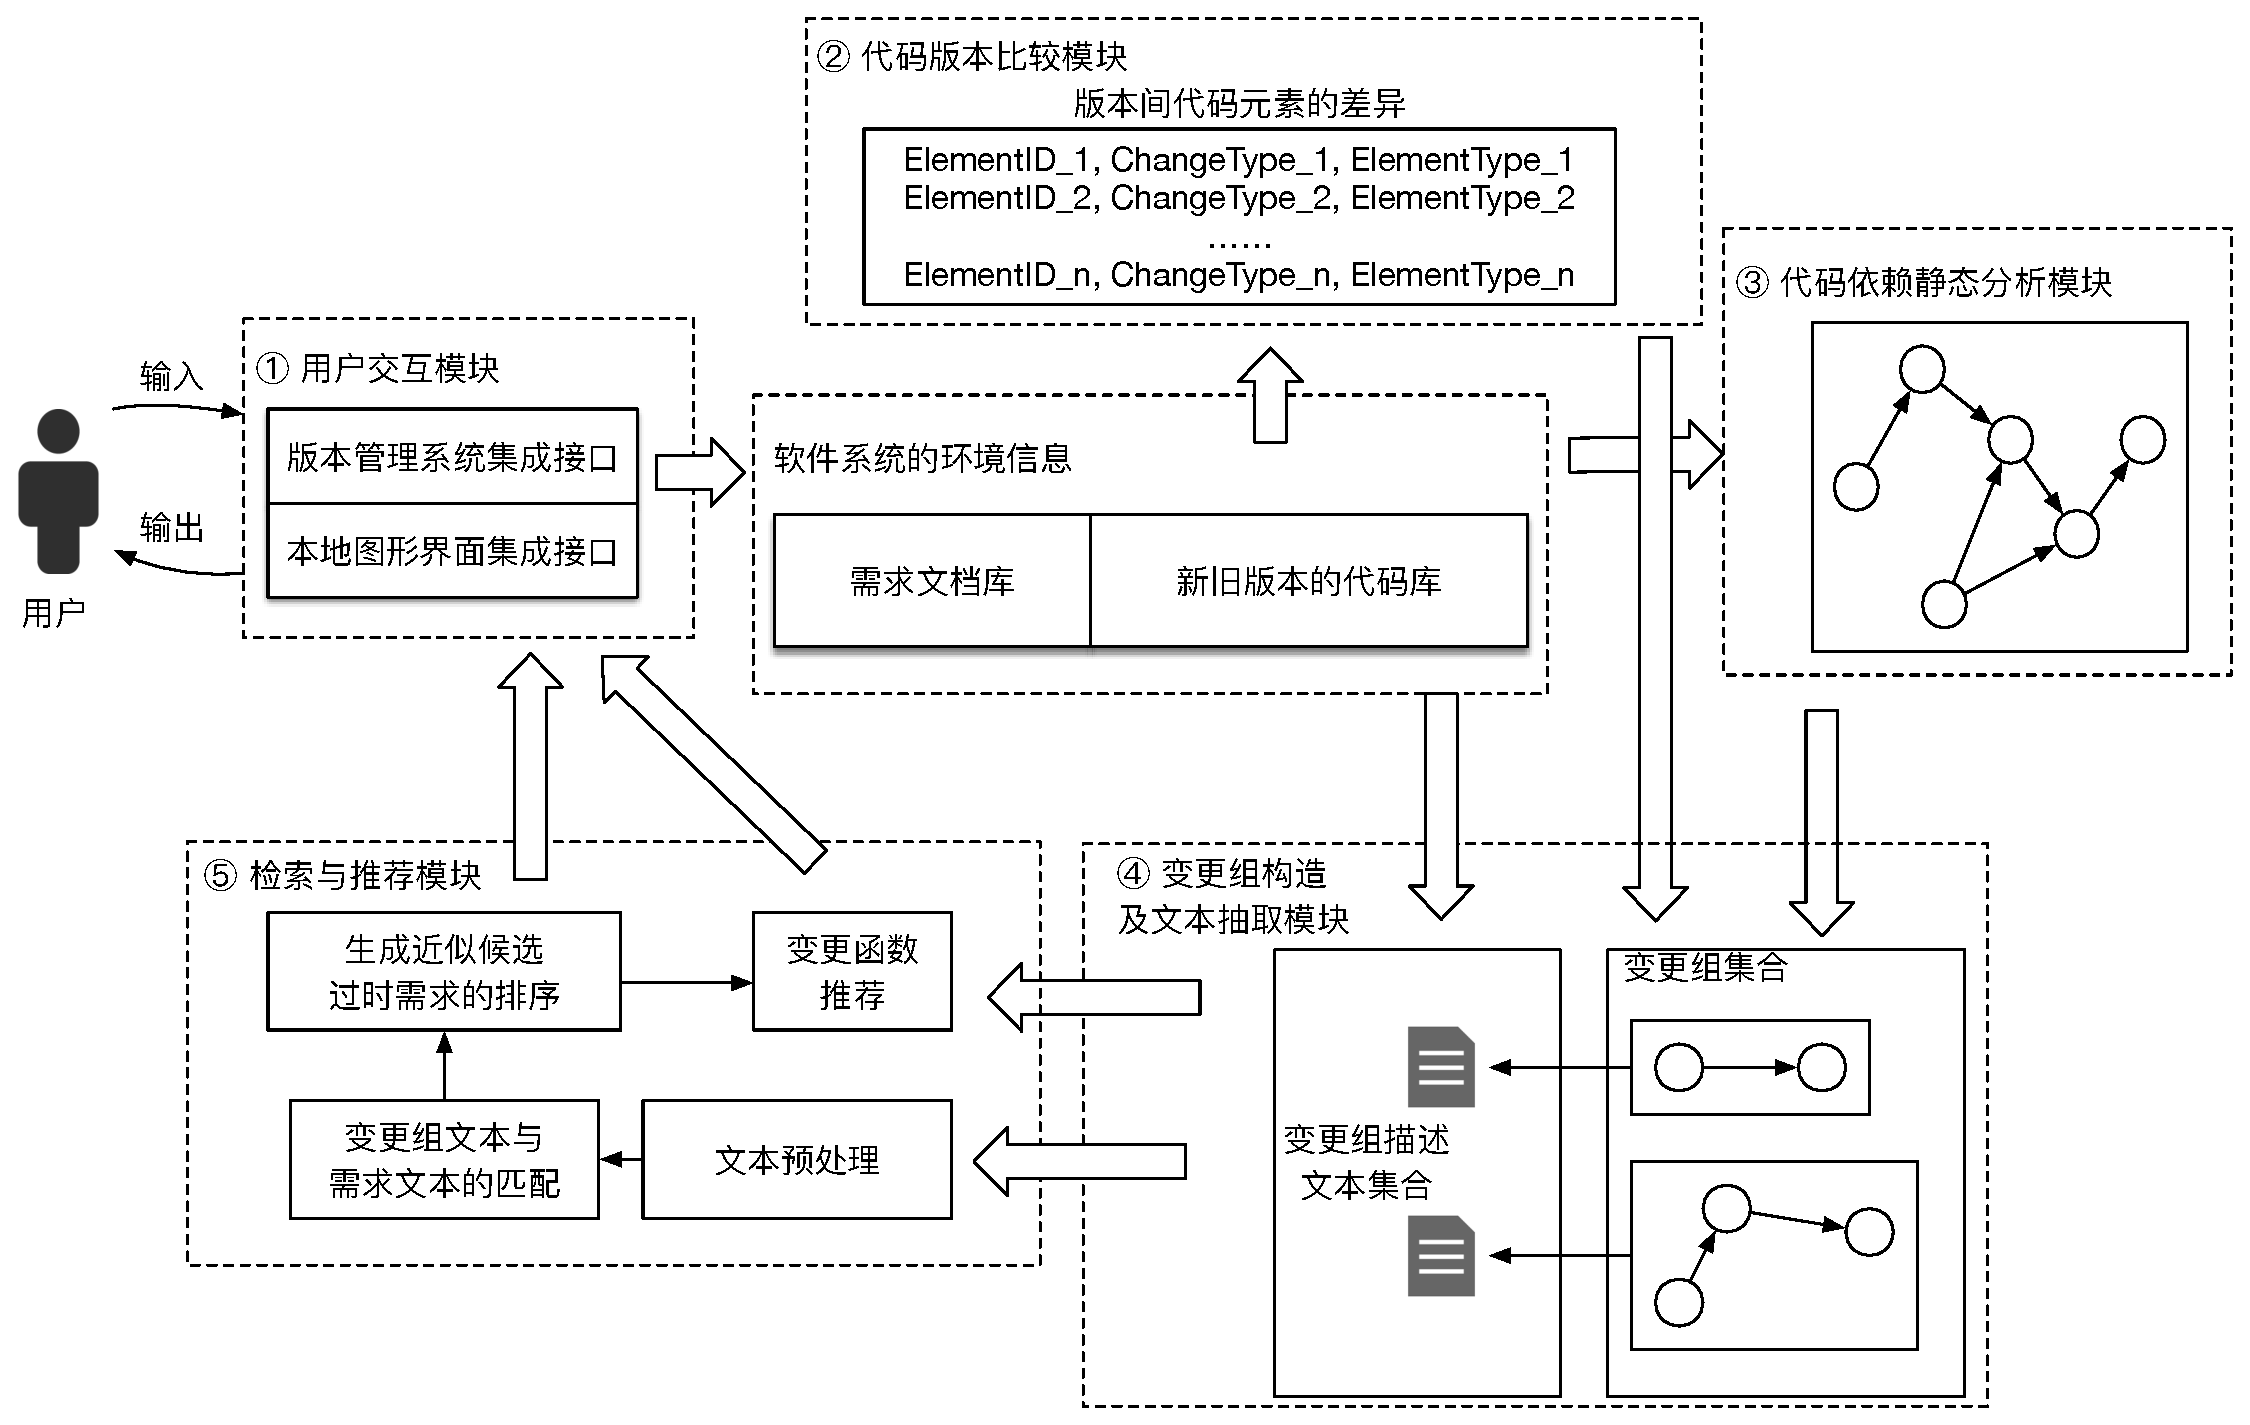
\includegraphics[width=1.0\textwidth]{./figures/inform/INFORM_Architecture.pdf}
    \caption{INFORM的系统体系结构图}
    \label{F:INFORM_Architecture}
\end{figure}

\begin{enumerate}
  \item 用户交互模块:INFORM通过此模块与用户(通常是维护人员)进行交互。用户较为熟悉的工具使用方式是图形界面或控制台,因此,INFORM的交互模块包含GUI与Console两个部分,它们共享同样的内核接口。

  以GUI版本的INFORM为例,对于任意一个软件项目,用户可以在文件系统中,指定需求,更新前后代码版本的路径,INFORM可以识别新旧版本间的代码元素差异并给予展示,用户此时可以通过点击界面的Retrieving按钮,以检测候选过时需求,检测结果将展示在当前界面的右上侧区域(如图N所示)。此外,用户可以选中其中的候选过时需求,并查看与该需求更新相关的变更函数的推荐,推荐结果展示在界面的左上侧区域。在GUI版本的INFORM的实现中,我们基于SWT(The Standard Widget Toolkit)完成了用户界面的设计,SWT提供了丰富的界面组件,能够满足INFORM的设计需要。

  对于Console版本的INFORM,我们将其与GitHub的接口相集成。用户只需提供项目的GitHub地址,需求的相对地址,并指定更新前后的代码版本号(CommitID),INFORM即可执行过时需求自动检测。
  \item 代码版本比较模块:在此模块中,INFORM比较了新旧两个版本代码间的差异,识别出其中的变更代码元素(包,类,函数,域)。在此过程中,我们基于Eclipse JDT(Java Development Tools)提取了源代码中的代码元素,并构造新旧版本的代码元素集合,通过比较集合间元素的不同,以识别出变更代码元素。

  \item 代码依赖静态分析模块:该模块主要负责代码依赖关系的抽取,其中包括函数的调用依赖及域的使用依赖。根据函数调用依赖的来源不同,对函数调用依赖的抽取有以下两种途径:(1)从编译后的字节码(Jar包)中抽取;(2)直接从代码的源文件(.Java为后缀的文件)中抽取。在前者的情况下,我们在静态分析时利用Apache BCEL库,析编译后的字节码以捕获代码的函数调用依赖。然而,在项目仓库中,对源码进行编译后产生的Jar文件通常是不可得的;在后者的情况下,经过我们的调研,没有发现能够直接从代码的源文件中抽取函数调用依赖的工具或类库。因此,我们基于Eclipse JDT对源码进行分析,实现了JDA(Java Dependencies Analyzer)工具,JDA可以直接分析代码的源文件并抽取函数调用依赖。域的使用依赖可以基于正则表达式的匹配获得。

  \item 变更组构造及文本抽取模块:首先,该模块基于获取的代码依赖关系,通过代码元素依赖的紧密度分析,可以获取与变更代码元素结构上紧密依赖的其他代码元素,以构成变更组。然后,模块根据变更组中代码元素的不同来源抽取关键词,从而构造变更组文本。通过词形还原,词根提取(Snowball Stemming)和去停用词等预处理技术标准化文本。

  \item 检索与推荐模块:
  在检索部分,该模块利用信息检索模型,计算变更组文本与需求文本的相似度矩阵,按照文本间相似度值发现近似候选过时需求。在此部分中,我们实现了词项-文档矩阵(TermByDocumentMatrix),相似度矩阵(SimilarityMatrix)等基础数据结构,以及VSM,JS与LSI这三个被广泛使用的信息检索模型。在推荐部分,结合代码依赖关系信息,模块基于TF-IDF的赋权技术,通过计算变更代码元素标识符中词汇的全局重要性和局部重要性以获取该变更代码元素的重要性,进行热点元素的推荐(详见x.x.x节)。
\end{enumerate}

\section{案例分析}

\section{运行时系统行为}

\section{本章小结}

\chapter{总结与展望}

\section{工作总结}

\section{研究展望}



%%%%%%%%%%%%%%%%%%%%%%%%%%%%%%
%% 附件部分
%%%%%%%%%%%%%%%%%%%%%%%%%%%%%%
\backmatter

% 致谢
% \begin{thanks}
% \vskip 18pt

% 时光荏苒,转眼间已经要跟南大说再见了,在南大的三年研究生学习,让我在学识、做事以及做人三个方面都收获颇多。回顾这三年的成长,点点滴滴都离不开老师、朋友以及家长的帮助。现在,我即将踏入社会,在这之前,我想对这些年一路陪伴以及帮助我的人表示感谢。

% 首先感谢我的导师,胡昊老师。在研究生的三年中,胡老师无论是在学习上,还是在生活上都给予了我悉心的指导与关怀。胡老师在平时既是一个前辈,在人生规划、职场生活方面给了我很多宝贵的建议;又是一位益友,在一起讨论科研问题,探讨项目经验,让我在学术以及项目上面都得到很多的启发。从胡老师那里学得的,不仅是做事,更是做人,让我终身受益。

% 感谢宋巍老师,在科研上给了我很大的帮助,尤其两篇小论文的选题、成文、修改、定稿都离不开宋老师的帮助与教导。宋老师严谨学术风格以及科研素养让我受益颇多。

% 感谢曹春老师、余萍老师在我科研项目上的指导和帮助。感谢吕建教授、陶先平教授、马晓星教授、徐峰教授、许畅副教授、黄宇副教授、葛季栋老师、张建莹老师等所有关心和帮助过我的人。

% 感谢一起奋斗的同门,他们是张浩、王晶、陈栋、陶骏、张诚、戚可生、梁阳、聂佳、龚宇豪、单苏苏、卜琪,三年的成果离不开他们的帮助,希望大家以后都能有好的发展。感谢曹流师兄,在研一期间非常有耐心的指导我的科研项目,也祝愿师兄家庭和睦,事业有成。

% 感谢我的舍友方铭、邓晨,感谢他们这三年对我的照顾与包容。时间虽短,但是与你们的友谊我将一生珍惜。感谢好友赵博文,我会永远记得你在工作日放弃休息陪我通宵修改论文,深厚的友谊,我将一生铭记。

% 最后我要向我的家人致以最衷心的感谢和最诚挚的敬意。感谢父母对我的养育之恩,没有你们,不可能有我的今天。感谢我的女朋友陆雅君,从本科阶段就一直陪伴在我身旁,在我最无助困难的时候,总会给我鼓励,帮助我走出困境。感谢女朋友的父母,他们在生活上给予了我很多的照顾,让我在南京依然可以感受到家的温暖。他们是我一生珍贵的财富。

% 寥寥数语,无法表达我的全部感激。在以后的日子里,我将铭记感恩,继续努力,肩负着大家的期望,披荆斩棘,勇往直前。
% \end{thanks}

%个人简介
\Nchapter{简历与科研成果}
\noindent {\heiti 基本情况}
\vspace{1ex}
\noindent 聂佳,男,汉族,1990~年~12~月出生,江苏省苏州市人。
\vspace{2ex}

\noindent {\heiti 教育背景}
\begin{description}[labelindent=0em, leftmargin=8em, style=sameline]
\item[2013.9~2016.6] 南京大学计算机科学与技术系 \hfill 硕士
\item[2009.9~2013.6] 南京大学金陵学院计算机科学与技术 \hfill 本科
\end{description}

% 发表文章目录

\noindent {\heiti 攻读硕士学位期间发表的论文}

\begin{enumerate}[label=\arabic*., labelindent=0em, leftmargin=*]
	\item \textbf{Yu Du}, Hao Hu, Wei Song, Junhua Ding and Jian L\"{u}. Efficient Computing Composite Service Skyline with QoS Correlations. In \emph{Proceedings of International Conference on Services Computing}, 2015, Accepted.
    \item \textbf{Yu Du}, Hao Hu, Wei Song, Yuhao Gong and Jian L\"{u}. Safety-Range Aware Mobile Composite Service Skyline. In \emph{Proceedings of International Conference on Mobile Services}, 2015, Accepted.
\end{enumerate}

\noindent {\heiti 攻读硕士学位期间申请的专利}

\begin{enumerate}[label=\arabic*., labelindent=0em, leftmargin=*]
	\item 胡昊,宋巍,葛季栋,吕建,\textbf{杜宇},``一种计算具有QoS关联关系的QoS最优组合服务限定范围的方法'',申请号:201510168726.0,已授权。
\end{enumerate}

\vspace{4ex}
\noindent {\heiti 攻读硕士学位期间参与的科研课题}

\begin{enumerate}[label=\arabic*., labelindent=0em, leftmargin=*]
	\item 国家973计划:持续演进的自适应网构软件模型、方法及服务质量保障。项目编号No.2015CB352202。
\end{enumerate}
% 参考文献
\bibliography{./reference}

\end{document}

